\documentclass[
    left=2.5cm,         % Sadly, generic margin parameter
    right=2.5cm,        % doesnt't work, as it is
    top=2.5cm,          % superseded by more specific
    bottom=3cm,         % left...bottom parameters.
    bindingoffset=6mm,  % Optional binding offset.
    nohyphenation=false % You may turn off hyphenation, if don't like.
]{eiti/eiti-thesis}
\langpol % Dla języka angielskiego mamy \langeng
\graphicspath{ {img/} }

\renewcommand{\vec}[1]{\mathbf{#1}}
\renewcommand{\function}[1]{\texttt{#1}}
\DeclareMathOperator{\argmin}{\operatorname*{argmin}} % thin space, limits on side in displays
\DeclareMathOperator{\argmax}{\operatorname*{argmax}} % thin space, limits on side in displays


\begin{document}

\EngineerThesis % Dla pracy inżynierskiej mamy \EngineerThesis
\instytut{Instytut Automatyki i Informatyki Stosowanej}
\kierunek{Informatyka}
\specjalnosc{Systemy Informacyjno-Decyzyjne}
\title
{
    Aplikacja do testowania odporności modeli klasyfikacyjnych \\
    na ataki z użyciem złośliwych danych \\
}

\engtitle
{ % Tytuł po angielsku do angielskiego streszczenia
    Unnecessarily long and complicated thesis' title \\
    difficult to read, understand and pronounce
}

\author{Jan Ambroziak}
\album{269260}
\promotor{dr inż. Paweł Zawistowski}
\date{\the\year}
\maketitle

%--------------------------------------
% Streszczenie po polsku
%--------------------------------------
\cleardoublepage % Zaczynamy od nieparzystej strony
\streszczenie \lipsum[1-3]
\slowakluczowe XXX, XXX, XXX

%--------------------------------------
% Streszczenie po angielsku
%--------------------------------------
\newpage
\abstract \kant[1-3]
\keywords XXX, XXX, XXX

%--------------------------------------
% Oświadczenie o autorstwie
%--------------------------------------
\cleardoublepage  % Zaczynamy od nieparzystej strony
\pagestyle{plain}
\makeauthorship

%--------------------------------------
% Spis treści
%--------------------------------------
\cleardoublepage % Zaczynamy od nieparzystej strony
\tableofcontents

%--------------------------------------
% Rozdziały
%--------------------------------------
\cleardoublepage % Zaczynamy od nieparzystej strony
\pagestyle{headings}

\section{Wstep}
Choć pierwsze wzmianki o perceptronie pojawiają się w publikacjach jeszcze z lat 50~\cite{TIBKAT:271027045},
a o splotowych sieciach neuronowych w latach 80\cite{doi:10.1162/neco.1989.1.4.541}, to ostatnia dekada przyniosła bezprecedensowy skok w zainteresowaniu
tematem zastosowania sieci neuronowych w związku z klasyfikacją obrazów.
Od momentu gdy głęboka splotowa sieć neuronowa AlexNet~\cite{NIPS2012_4824} wygrała edycję konkursu ILSVRC~\cite{ILSVRC15} w 2012 roku sieci neuronowe stały się
dominującą techniką klasyfikacji obrazów.
Współczesne modele korzystają z zdecydowanie bardziej zaawansowanych technik oraz są rzędy wielkości większe
od wspominanych prekursorów.
Jako dobry przykład skoku jakościowego można potraktować wyniki jakie modele osiągają w klasyfikacji zbioru ImageNet~\cite{ILSVRC15} czy pokrewnego ImageNet-v2~\cite{DBLP:journals/corr/abs-1902-10811}.
W 2011 precyzja top-1 najlepszych modeli, nie opierających się na sieciach neuronowych, znajdowała się w okolicach 50\%, natomiast
opisana w Kwietniu bieżącego roku, sieć FixEfficientNet-L2~\cite{Touvron2020FixingTT} osiąga, dla zbioru ImageNet-v2 precyzję top-1 na poziomie około 88.5\%
Pozwoliło to na rozwiązanie szeregu wcześniej skomplikowanych problemów, takich jak automatyzacja diagnostyki obrazów medycznych,
rozwój autonomicznych pojazdów, czy wachlarz technik biometrycznej identyfikacji.

Wraz z rozwojem i upowszechnianiem się modeli klasyfikujących obrazy,
pojawiają się nowe zagrożenia związane z bezpieczeństwem tej klasy rozwiązań.
Jednym z nich są złośliwe dane, które mogą powodować,
że pozornie dobrze działający klasyfikator zaczyna udzielać błędnych odpowiedzi.
Może to stanowić realne zagrożenie nawet dla życia i zdrowia ludzkiego.
Od momentu publikacji artykułu \textit{Intriguing properties of neural networks}~\cite{DBLP:journals/corr/SzegedyZSBEGF13} w 2014 roku,
w którym autorzy opisali pierwszą metodę tworzenia złośliwych danych, w środowisku zajmującym się tematyką nauczania maszynowego można zaobserwować swojego rodzaju
''wyścig zbrojeń'' w poszukiwaniu nowych metod, obrony przed i generowania adwersaryjnych przykładów.

\subsection{Cel}
\label{sec:target}

Celem pracy inżynierskiej jest stworzenie aplikacji która ma wspierać testowanie
odporności modeli klasyfikacyjnych na ataki z użyciem złośliwych danych
Dla dostarczonego w narzuconej postaci modelu klasyfikatora możliwe będzie
przeprowadzenie ataku przy pomocy jednej z dostępnych metod.

\subsection{Istniejące rozwiązania}

Aktualnie na rynku znajduje się kilka rozwiązań implementujących podobne funkcjonalności
do tej która jest tu opisana. Warto zapoznać się z nimi oraz ich implementacjami.
Jednym z najbardziej popularnych narzędzi tego typu jest \textit{CleverHans}\cite{DBLP:journals/corr/GoodfellowPM16}
wykorzystujący jako swoją bazę framework TensorFlow oraz \textit{Adversarial Robustness Toolbox}\cite{DBLP:journals/corr/abs-1807-01069} opracowany przez IBM.
Ciekawym przypadkiem jest też biblioteka \textit{Foolbox}\cite{rauber2017foolbox} która dostarcza natywne wsparcie dla wykorzystywanych frameworków.

%\subsection{Użyte narzędzia}
%Od czasu opublikowania przez firmę Google biblioteka TensorFlow~\cite{DBLP:journals/corr/AbadiABBCCCDDDG16}
%stała się jednym z wiodących narzędzi wykorzystywanych w branży. Prostota API i intuicyjność
%języka Python, akceleracja obliczeń z wykorzystaniem procesorów graficznych oraz dobra integracja z
%popularnymi bibliotekami dostępnymi dla języka Python czyni TensorFlow idealnym kandydatem.
%W trakcie pracy wykorzystywałem głównie wysokopoziomowy interfejs Keras, który pozwala na szybkie
%prototypowanie przez wysoki poziom abstrakcji jaki zapewnia. Keras zapewnia nam też dostęp do wytrenowanych modeli takich
%InceptionV3~\ref{InceptionV3} i MobileNetV2~\ref{MobileNetV2}, których wytrenowanie na potrzebę naszych testów byłoby
%trudne z uwagi na ich złożoność.
%Platforma testowa jakiej użyto to:
%\begin{itemize}
%    \item CPU: AMD Ryzen 3900X
%    \item GPU: Nvidia GeForce 1060 GTX 6GB
%    \item RAM: 32GB DDR4
%    \item System Operacyjny: Windows 10
%    \item Tensorflow wersja 2.2.0
%    \item Interpreter Python 3.6.8 wersja 64bit
%\end{itemize}
%Wszystkie pozostałe biblioteki Python, wraz z wersjami, wykorzystane w projekcie, znajdują się w pliku
%requirements.txt w folderze projektu.

\newpage

\section{Złośliwe Dane}
W związku z dużym rozwojem uczenia maszynowego (z ang. Machine Learning) w ostatnich latach i zastosowaniem go do
rozwiązania problemów w których poprawne funkcjonowanie jest krytyczne. Zagadnienie bezpieczeństwa tego typu rozwiązań stało
się niezwykle istotne. Szereg publikacji z ostatnich lat pokazał martwiące luki w działaniu popularnych technik.
Jedną z pierwszych tego typu publikacji jest, udostępniona w 2014 roku, \textit{Intriguing properties of neural networks}\cite{DBLP:journals/corr/SzegedyZSBEGF13},
która pokazała skuteczną metodę ataku, która wykorzystywała małą zmianę w przykładzie wejściowym klasyfikatora aby zmienić wynik klasyfikacji.
Przygotowane w ten sposób złośliwe przykłady (z ang. adversarial examples), zawierające specjalnie przygotowaną perturbacje,
choć dla ludzkiego oka, praktycznie nieodróżnialne od oryginału, są w stanie skutecznie oszukać klasyfikatory co możemy zaobserwować na rysunku ~\ref{intrguing_plot}.
Warto też dodać że choć popularne modele splotowych sieci neuronowych są stosunkowo odporne na niewielki losowy szum~\cite{DBLP:journals/corr/abs-1807-10108}, to wykazują niską odporność na omawiane przez nas ataki.

Implikacje dla bezpieczeństwa, na przykład, systemu rozpoznawania obrazów autonomicznego pojazdu są poważne co
pokazano w kilku osobnych publikacjach~\cite{DBLP:journals/corr/EvtimovEFKLPRS17,DBLP:journals/corr/abs-1907-00374, DBLP:journals/corr/abs-1801-02780}.
Kolejne prace starały się rozwinąć wachlarz metod ataków, oraz metod obrony\cite{DBLP:journals/corr/PapernotMWJS15, DBLP:journals/corr/abs-1801-08926, DBLP:journals/corr/abs-1904-00887} które pokrótce opisujemy w rozdziale~\ref{secition:metody_obrony}.
\begin{figure}[h]
    \begin{center}
        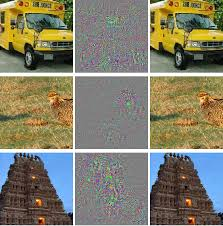
\includegraphics[width=0.75\linewidth]{eiti/adversarial_intriguing.jpg}
    \end{center}
    \caption{Przykład z \textit{Intriguing properties of neural networks}\cite{DBLP:journals/corr/SzegedyZSBEGF13}.
        W lewej kolumnie: poprawnie klasyfikowane oryginalne obrazy, w środkowej: dodana do obrazów perturbacja, w prawej: obrazy z perturbacją klasyfikowane jako struś}
    \label{intrguing_plot}
\end{figure}

Możemy opisać złośliwy atak jako funkcję:
\begin{equation}
    q(\vec{x}, f)=\vec{x'} \text{ taką że } f(\vec{x'})=\widetilde{y} \text{ lub } f(\vec{x'})\neq{y},
\end{equation}
gdzie $\vec{x}$ to wektor wejściowy, $f()$ to funkcja opisująca nasz model klasyfikacyjny, $\vec{x'}$ to wektor reprezentujący wygenerowany złośliwy przykład,
$y$ to prawdziwa klasa do której należy przykład wejściowy, a $\widetilde{y}$ to zadana klasa z którą chcemy żeby model sklasyfikował nasz złośliwy przykład.
Większość metod stara się także minimalizować wprowadzoną do obrazy perturbacje:
\begin{equation}
    \|\vec{x}-\vec{x'}\|_2 < \epsilon \text{  lub  } \min \|\vec{x}-\vec{x'}\|_2.
\end{equation}
Powyższe definicje z uwagi na różnorodność ataków sa opisem dość upraszczającym faktyczną sytuację.
Cele naszego ataku mogą być różne, tak samo jak i dostępna dla atakującego wiedza (np. znajomość modelu $f()$ czy dostępność przykładu wejściowego $\vec{x}$) opisujemy to szerzej w podrozdziale~\ref{attack-kinds}.

Przyczyna skuteczności i istnienia złośliwych danych nie jest znana i wydaje się nie być łatwym problemem do rozwiązania.
Natomiast istnieje kilka hipotez starających się wyjaśnić to zjawisko.
Autorzy \textit{Explaining and Harnessing Adversarial Examples}~\cite{harnessing} sugerują że skuteczność złośliwych danych wynika z zbytniej liniowości modeli klasyfikacyjnych.
i jest konsekwencją iloczynu skalarnego liczonego w warstwach ukrytych sieci dla wysoko wymiarowych danych.
Natomiast w publikacji \textit{Adversarial examples from computational constraints}~\cite{Bubeck2019AdversarialEF},
zaproponowano że istnienie złośliwych danych jest wynikiem ograniczeń spowodowanej przez wysoką złożoność obliczeniową współczesnych technik nauczania maszynowego.
Autorzy usiłują wykazać że wytrenowanie modelu który byłby odporny na ataki jest możliwe, lecz bardzo kosztowne obliczeniowo i przez to trudne.
Hipoteza zaproponowana w \textit{Intriguing properties of neural networks}~\cite{DBLP:journals/corr/SzegedyZSBEGF13} zakłada
że skuteczność ataku proponowanego przez autorów jest konsekwencją nieciągłości modelu, wbrew wcześniejszym założeniom dotyczącym metod wykorzystujących filtry splotowe.
%TODO Tutaj można dodać wzór z wyjasnieniem z Explaining and Harnessing tłumaczący argument o liniowości
%TODO Można też dodać przykład z tego https://arxiv.org/pdf/1901.10861.pdf

\newpage

\subsection{Rodzaje Ataków}\label{attack-kinds}
Autorzy \textit{The Limitations of Deep Learning in Adversarial Settings}~\cite{DBLP:journals/corr/PapernotMJFCS15}
dokonali bardzo pomocnego podziału ataków w dwóch kategoriach - dostępnych danych oraz narzuconego atakowi celu. Tak określony
model zagrożenia (z ang. thread model) pozwala nam na klarowny podział ataków i zrozumienie ich przeznaczenia. Warto też dodać
że nie wszystkie ataki starają się minimalizować perturbację $\vec{r}$ czy też modyfikować przykłady wejściowe. Opublikowane zostały
metody ataków wykorzystujących algorytmy ewolucyjne które generują złośliwe dane niezależne od danych wejściowych i nie starające się
imitować przykładów ze zbioru danych. Przykładem publikacji w którym opisany został tego typu atak jest \textit{Deep Neural Networks are Easily Fooled: High Confidence Predictions for Unrecognizable Images}~\cite{DBLP:journals/corr/NguyenYC14}.
\\~\\
Narzucone cele ataku możemy uporządkować zgodnie z rosnącą trudnością zadania.
\begin{enumerate}
    \item Zmniejszenie prawdopodobieństwa z jakim model klasyfikuje przykład jako należący do prawdziwej klasy.
    \item \label{cel_ataku_2} Zła klasyfikacja przykładu wejściowego bez zadanej z góry przez atak klasy. Takie ataki nazywamy nieukierunkowanymi(z ang. untargeted), bądź atakami bez zadanej klasy.
    \item Wygenerowanie przykładu który zostanie przyporządkowany do zadanej z góry klasy.
    \item \label{cel_ataku_4} Zmodyfikowanie istniejącego już przykładu który zostanie przyporządkowany do zadanej z góry klasy. Takie ataki nazywamy ukierunkowanymi(z ang. targeted), bądź atakami z zadaną klasą.
\end{enumerate}
Omawiane przez nas poniżej ataki są w stanie osiągnąć cel~\ref{cel_ataku_4} bądź cel~\ref{cel_ataku_2} z tych opisanych powyżej.
\\~\\
Możemy też rozróżnić ataki z uwagi na to jakie dane są dostępne dla algorytmu atakującego:
\begin{enumerate}
    \item \label{atak_1} Dostępna jest pełna wiedza o modelu który atakujemy. Jego architektura, dane treningowe, sposób trenowania, wartości parametrów dla wszystkich warstw etc.
    \item \label{atak_2} Dostępna jest tylko tylko architektura modelu i wartości parametrów.
    \item Dostępny jest podzbiór zbioru danych używanych do wytrenowania modelu.
    \item Dostępny jest model w postaci czarnej skrzynki. Otrzymujemy tylko klasyfikacje na podstawie dostarczonych przez nas przykładów.
    \item Dostępne są tylko pary w postaci (\textit{Przykład}, \textit{Wyjście Modelu}).
\end{enumerate}
W myśl tego rozróżnienia SimpleNet CIFAR-10~\ref{SimpleNetCIFAR-10}, SimpleNet CIFAR-100~\ref{SimpleNetCIFAR-100},
LeNet5~\ref{LeNet5} i Model Splotowy~\ref{MNIST_TF} w przypadku naszych ataków należą do kategorii~\ref{atak_1} jako że są zdefiniowane i wytrenowane przez nas w aplikacji.
Natomiast modele MobileNetV2~\ref{MobileNetV2} i InceptionV3~\ref{InceptionV3} do kategorii~\ref{atak_2}, ponieważ korzystamy z dostarczonych przez bibliotekę Keras wytrenowanych wag i implementacji.

\begin{figure}[H]
    \begin{center}
        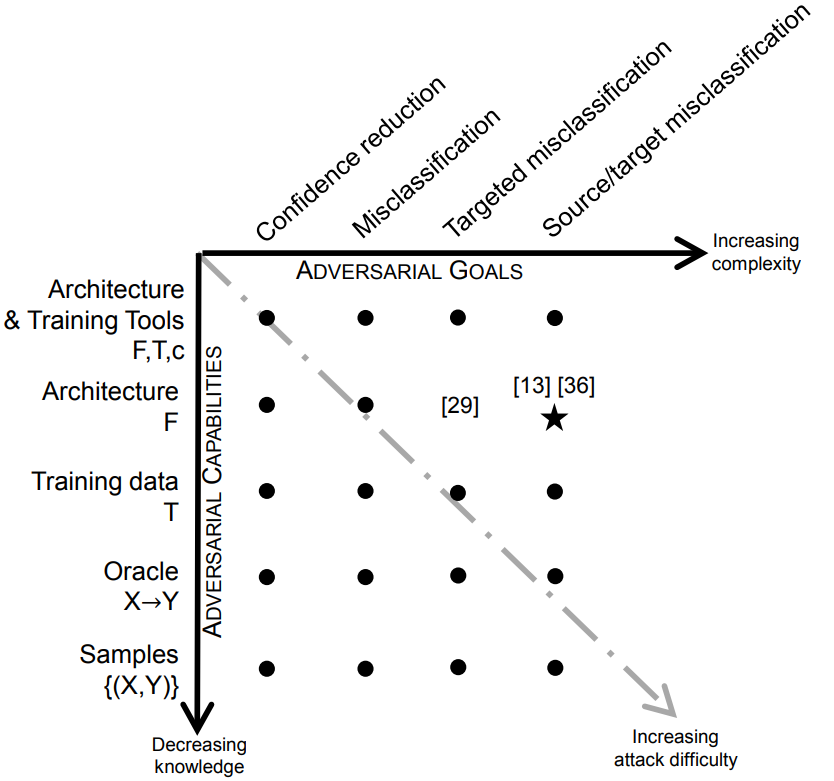
\includegraphics[width=0.75\textwidth]{eiti/attacks_taxonomy.png}
    \end{center}
    \caption{Ilustracja powyższego podziału ataków z oryginalnej publikacji~\cite{DBLP:journals/corr/PapernotMJFCS15}}
\end{figure}

\newpage

\subsection{Metody Obrony}\label{secition:metody_obrony}
Jak wspomniano wcześniej, istotną częścią zagadnienia ataków na modele klasyfikacyjne z użyciem złośliwych danych są
także techniki obrony przed nimi. Warto tu wspomnieć o kilku metodach obrony przed atakami które zostały
zaproponowane w publikacjach.
\begin{description}
    \item[Trenowanie Adwersaryjne]
    Trenowanie Adwersaryjne (z ang. Adversarial Training)\cite{DBLP:journals/corr/abs-1712-07107} to termin opisujący szeroką gamę technik obrony które posiadają
    zasadniczą cechę wspólną - wykorzystują złośliwe przykłady i metody ich generacji w procesie trenowania.
    Podstawowa idea polega tego zestawu metod polega na optymalizacji problemu min-max zadanego w następujący sposób.
    \begin{equation}
        \min _{\theta} \max _{\|(\vec{x}, \vec{x'})\|_2<\eta} J(\theta, \vec{x'}, y)
    \end{equation}
    gdzie człon $\min$ stara się zminimalizować błąd modelu klasyfikacyjnego poprzez modyfikacje parametrów $\theta$, a człon $\max$ stara się znaleźć
    złośliwe przykłady maksymalizujące funkcję kosztu $J$.
    \item[Różnorodne Trenowanie Adwersaryjne]
        Różnorodne Trenowanie Adwersaryjne (z ang. \textit{Ensemble adversarial training}) czy też EAT. Opisane w \textit{Ensemble Adversarial Training: Attacks and Defenses}~\cite{Tramr2018EnsembleAT} to rozwinięcie
        techniki Trenowania Adwersaryjnego. W tym przypadku zamiast dokonywać kosztownego Trenowania Adwersaryjnego,
        które musi w każdej treningowej iteracji wygenerować złośliwy przykład oraz przeprowadzić standardową propagację wsteczną w sieci,
        trenujemy model korzystając ze zbioru wygenerowanych (dla różnych modeli) a priori złośliwych przykładów.
        To podejście oprócz próby zmniejszenia kosztów obliczeniowych związanych z klasycznym trenowaniem adwersaryjnym, ma na celu
        zmniejszenie szans powodzenia atak black-box korzystającego z przykładów wygenerowanych dla innego modelu.
    \item[Modyfikacja przykładów]
        Głębokie splotowe sieci neuronowe zazwyczaj są dość odporne na losowe zmiany wektora wejściowego.
        Modyfikacja potencjalnie złośliwych przykładów wejściowych ma na celu ``zatracenie'' zmian adwersaryjnych w losowej modyfikacji obrazu,
        które w normalnych warunkach nie mają znacznego wpływu na precyzję klasyfikacji.
        Publikacje opisujące ten temat podają szereg różnych metod takich jak na przykład zmiana rozmiarów obrazu~\cite{DBLP:journals/corr/abs-1711-01991} czy
        wprowadzenie przed każdą warstwą splotową warstwy zaszumiającej wektor wejściowy warstwy~\cite{DBLP:journals/corr/abs-1712-00673}.
    \item[Maskowanie Gradientu]
        Idea maskowania gradientu opisana oryginalnie w \textit{Practical Black-Box Attacks against Deep Learning Systems using Adversarial Examples}~\cite{DBLP:journals/corr/PapernotMGJCS16},
        stara się utrudnić bądź uniemożliwić obliczenie gradientu obrazu wejściowego względem wektora wyjściowego modelu.

        Przykładem techniki starającej się obfuskować gradient jest destylacja defensywna (z ang. deffensive distillation) opisana w
        \textit{Distillation as a Defense to Adversarial Perturbations against Deep Neural Networks}\cite{DBLP:journals/corr/PapernotMWJS15}.
        Opiera się ona na trenowaniu dwóch modeli.
        Pierwszy trenujemy z wykorzystaniem oryginalnych etykiet z zbioru wejściowego.
        Drugi natomiast w procesie trenowania jako etykiety przyjmuje wektor wyjściowy produkowany przez pierwsza sieć dla danego przykładu wejściowego.

        Z maskowaniem gradientu wiązano nadzieje w związku z rozwiązanie problemu ataków wykorzystujących gradient. Niestety pomimo kilku obiecujacych publikacji
        okazała się być znacząco mniej skuteczna niż oryginalnie zakładano.
        Autorzy \textit{Obfuscated Gradients Give a False Sense of Security: Circumventing Defenses to Adversarial Examples}~\cite{DBLP:journals/corr/abs-1802-00420},
        wykazują nieskuteczność tej klasy metod, pokazując dla kilku popularnych wariantów skuteczne ataki ignorujące niedostępność gradientu w modelach.
        Przykładem tego jest trenowanie modeli na tych samych, bądź podobnych zbiorach danych oraz tworzenie dla nich złośliwych przykładów.


\end{description}
Oczywiście nie opisujemy tutaj wszystkim możliwych metod obrony, a jedynie te najbardziej popularne. Każda z wspomnianych powyżej metod posiada co najmniej kilka
wariantów opisanych w osobnych publikacjach.
\newpage

\section{Implementacja}
Głównym założeniem w trakcie projektowania aplikacji była implementacja algorytmów wykorzystywanych do
tworzenia złośliwych przykładów, tak aby mogły być one w prosty sposób wykorzystywane przez użytkowników oraz zapewniały
wysoką wydajność przez korzystanie z akceleracji za pomocą GPU.
Język skryptowy Python stał się lingua franca w dziedzinie nauczania maszynowego,
dlatego rozważania dotyczące biblioteki na której miała bazować nasza aplikacja zostały ograniczone do tych wspierających ten język.
Decyzja wyboru TensorFlow była podyktowana głównie łatwością użycia wysokopoziomowego interfejsu i popularnością. Nie mały wpływ na tą decyzję miało też to że
zapewnia akceleracje GPU oraz dostarcza API Keras które pozwala na łatwe portowanie modeli między bibliotekami Theano\cite{2016arXiv160502688short}, TensorFlow\cite{DBLP:journals/corr/AbadiABBCCCDDDG16} czy CNTK\cite{cntk}.
Aplikacja udostępnia też proste w użyciu funkcjonalności umożliwiające tworzenie zbiorów danych zawierających złośliwe przykłady.
Ze strony użytkownika wystarczy dostarczyć model zgodny z API Keras dostępnym w TensorFlow, aby móc wykonać wszystkie ataki
dostępne w bibliotece.

Szczegóły dotyczące korzystania z dostarczanej przez nas aplikacji, oraz uruchomienia znajdują się w załączonym pliku README.md

\begin{center}
    \begin{table}[ht]

    \caption{Porównanie bibliotek generujących złośliwe przykładu.}
    \begin{tabular}{|>{\centering}p{2.5cm}|>{\centering}p{2.5cm}|>{\centering}p{2.5cm}|p{7.0cm}|}
        \hline
        X & wsparcie GPU & Liczba Ataków & Wspierane frameworki\\
        \hline
        Foolbox & Tak\footnotemark[1] & \textasciitilde33 & PyTorch, TensorFlow, JAX, NumPy\\
        \hline
        CleverHans & Tak\footnotemark[1] & \textasciitilde12 & TensorFlow (JAX i PyTorch wkrótce)\\
        \hline
        Adversarial Robustness Toolbox & Tak\footnotemark[1] & \textasciitilde39 & TensorFlow, Keras, PyTorch, MXNet, scikit-learn, XGBoost, LightGBM, CatBoost, GPy \\
        \hline
        Nasza Biblioteka & Tak & 6 & TensorFlow\\
        \hline
    \end{tabular}
    \end{table}
\end{center}
\footnotetext[1]{Zależy od konkretnego frameworku}

\newpage



\section{Wykorzystane Ataki}
W projekcie zaimplementowanych zostało kilka popularnych ataków które zostały opisane w anglojęzycznych publikacjach.
Poniżej znajdują się ich opisy, uwagi dotyczące implementacji, przykłady zastosowania oraz wyniki testów
zastosowanych do oceny ataków. Szersza dyskusja dotycząca użyteczności oraz porównanie znajdują się w sekcji~\ref{comparison}

\subsection{FGSM}
    FGSM czyli Metoda szybkiego znaku gradientu (z ang. Fast Gradient Sign Method) opsiana w artykule
    pod tytułem \textit{Explaining and Harnessing Adversarial Examples}\cite{harnessing} to jedna z pierwszych
    opisanych metod ataku na modele klasyfikacyjne wykorzystujący złośliwe dane.
    Aby wygenerować złośliwy przykład metoda ta wymaga znajomości gradientu funkcji kosztu obliczanego względem danych
    wejściowych oznaczonego jako

    \begin{equation}
        \nabla_{x} J(\vec{x}, y),
    \end{equation}
    gdzie, $\vec{x}$ to wektor wejściowy, a $y$ to klasa do której należy wektor wejściowy.
    Idea metody polega na dodaniu bądź odjęciu małej, arbitralnie ustalonej, wartości  \(\epsilon\) do
    wektora wejściowego w kierunku znaku gradientu. Pozwala nam to zwiększyć wartość funkcji kosztu,
    doprowadzając do niepoprawnej klasyfikacji danych wejściowych zmodyfikowanych w niewielkim stopniu.


    Możemy zapisać to działanie w następujący sposób:
    \begin{equation}
    \vec{x'} = \vec{x} + \epsilon\operatorname{sign}(\nabla_{x} J(\vec{x}, y)),
    \end{equation}
    gdzie $\vec{x'}$ to spreparowany przykład ze złośliwymi danymi.

    Podstawową wadą opisywanej metody jest fakt że nie mamy wpływu na to jaka będzie klasa wyjściowa
    spreparowanych przez nas danych wejściowych. Kolejną jest to że niektóre dane i modele wymagają od nas
    doboru wysokiej wartości parametru $\epsilon$ aby być w stanie spreparować pożądane dane, co z kolei powoduje dużą
    różnicę między danymi wejściowymi a tymi utworzonymi w toku stosowania metody.
    W publikacji pod tytułem \textit{Adversarial examples in the physical world}\cite{DBLP:journals/corr/KurakinGB16}
    autorzy opisują kilka metod podobnych do FGSM.

    \subsubsection{I-FGSM}\label{ifgsm-algorith}
    I-FGSM czyli Iteracyjna Metoda Szybkiego Znaku Gradientu (z ang. Iterative Fast Gradient Sign Method) to metoda
    które rozwiązuje problem konieczności doboru wysokiej wartości $\epsilon$ poprzez zastosowanie metody FGSM kilkakrotnie,
    jednocześnie zapewniając pod koniec każdego kroku że przygotowany każdy piksel obrazu nie różni się od oryginału o więcej
    niż $\epsilon$, z niższą wartością parametru $\epsilon$ niż wymagane oryginalnie w metodzie jednokrokowej.
    Pozwala to  potencjalnie ograniczyć różnicę między preparowanymi przez nas danymi, a oryginalnymi danymi wejściowymi
    oraz przerwanie działania metody kiedy model przestanie poprawnie klasyfikować dane wejściowe.

    \begin{algorithm}
    \caption{I-FGSM}\label{IFGSM}
    \begin{algorithmic}[1]
    \State $i \gets 0$
    \State $\vec{x'} \gets \vec{x}$
    \While{$i <  i_{max}$}
        \State $\vec{x'} \gets \vec{x'} + \alpha\operatorname{sign}(\nabla_{x} J(\vec{x}, y))$
        \State $i \gets i+1$
        \State $\function{Przytnij}(\vec{x'}, \epsilon)$
    \EndWhile
    \end{algorithmic}
    \end{algorithm}

    Funkcja $\function{Przytnij}()$ ma na celu ograniczenie różnicy wartości atrybutów przykładu oryginalnego i przykładu złośliwego
    do co najwyżej $\epsilon$. Robimy to stosując dla każdego atrybutu wektora reprezentującego złośliwy przykład poniższą metodę.
    \begin{equation}
        \vec{x'}_i = \left\{
        \begin{array}{l r}
            \vec{x}_i + \epsilon & \text{ jeśli } \vec{x'}_i > \vec{x}_i + \epsilon \\
            \vec{x}_i - \epsilon & \text{ jeśli } \vec{x'}_i < \vec{x}_i - \epsilon \\
            \vec{x'}_i & \text{ jeśli } \vec{x}_i - \epsilon  < \vec{x'}_i < \vec{x}_i + \epsilon \\
        \end{array}
    \end{equation}

    \subsubsection{LL-FGSM}\label{llfgsm-algorithm}
    LL-FGSM (z ang. Least Likely FGSM) to metoda pozwalająca nam na spreparowanie danych które będę przydzielane do
    konkretnej klasy (ozn. $\vec{\widetilde{y}}$), a nie tylko na niepoprawną klasyfikacje. W tym wypadku zamiast starać się
    zmieniać wartości pikseli obrazu zgodnie z kierunkiem gradientu funkcji kosztu dla prawidłowej klasy
    staramy się zmieniać wartości pikseli przeciwnie do kierunku gradientu funkcji kosztu dla klasy $\vec{\widetilde{y}}$.
    Intuicyjnie można to opisać jako nie oddalanie się od prawdziwej klasy obrazu, a jako przybliżanie się do zadanej
    przez nas klasy.
    Autorzy metody zwracają uwagę na przydatność tej metody
    w przypadku gdy korzystamy z modeli operujących wieloma klasami i gdzie różnice między obiektami z różnych klas mogą
    być bardzo niewielkie (np. między rasami psów). Metoda ta jest także iteracyjna i zapewnie różnice między
    odpowiednimi pikselami obrazów nie większą niż $\epsilon$ więc można uznać ją za rozszerzenie metody I-FGSM.

    \begin{algorithm}
    \caption{LL-FGSM}\label{LLFGSM}
    \Input{\textbf{Input: }
    zadana klasa $\vec{\widetilde{y}}$ z którą chcemy żeby złośliwy przykład był klasyfikowany
    }
    \begin{algorithmic}[1]
    \State $i \gets 0$
    \State $\vec{x'} \gets \vec{x}$
    \While{$i <  i_{max}$}
        \State $\vec{x'} \gets \vec{x'} - \alpha\operatorname{sign}(\nabla_{x} J(\vec{x}, \vec{\widetilde{y}}))$
        \State $i \gets i+1$
        \State $\function{Przytnij}(\vec{x'}, \epsilon)$
    \EndWhile
    \end{algorithmic}
    \end{algorithm}

\subsection{DeepFool}
W publikacji \textit{DeepFool: a simple and accurate method to fool deep neural networks}\cite{DBLP:journals/corr/Moosavi-Dezfooli15}
autorzy proponują metodę alternatywną do FGSM mającą minimalizować wprowadzaną do danych wejściowych perturbacje jednocześnie
osiągając zmianę klasy do której model przyporządkowuje dane wejściowe.

Wadą DeepFool jest brak możliwości narzucenia klasy do której chcielibyśmy aby przyporządkowywane były nasze zmodyfikowane dane.
Metoda ta jest nieco bardziej złożona obliczeniowo jako że pojedynczy krok algorytmu wymaga od nas obliczenia gradientu dla
prawdopodobieństwa każdej klasy względem danych wejściowych, co przy zbiorach danych z wieloma klasami
takich jak np. ImageNet może być problematyczne. Poniżej znajduje się pseudokod opisujący metodę DeepFool dla modelu
wieloklasowego.
\begin{algorithm}
\caption{DeepFool}\label{DeepFool}
\Input{\textbf{Input: }
    oryginalny przykład $\vec{x}$,
    funkcja określająca model $f(\vec{x})$
}
\begin{algorithmic}[1]
\State $\vec{x^0} \gets \vec{x}$
\While{$f(\vec{x^{i}}) =  y$}
\For{$k \neq y$}
    \State $\vec{w'}_k\gets \nabla f_k(\vec{x}^i) - \nabla f_{y}(\vec{x}^i)$
    \State $f'_k\gets f_{k}(\vec{x}^i) - f_{y}(\vec{x}^i)$
\EndFor
\State $\hat{l}\gets \arg \min_{k\neq y} \dfrac{|f'_k|}{||\vec{w'}_k||_2}$
\State $r_i\gets \dfrac{|f'_{\hat{l}}|}{||\vec{w'}_{\hat{l}}||^2_2}\vec{w'}_{\hat{l}}$
\State $\vec{x}_{i+1}\gets \vec{x}_i + \vec{r}_i$
\State $i\gets i + 1$
\EndWhile
\State  $\hat{\vec{r}} = \sum_{i} \vec{r}_i$
\State  $\vec{x'} = \vec{x}_0 + \hat{\vec{r}}$
\State \textbf{return} $\vec{x'}$
\end{algorithmic}
\end{algorithm}




\subsection{L-BFGS-B}
Metoda opisana w \textit{Intriguing properties of neural networks}\cite{DBLP:journals/corr/SzegedyZSBEGF13}
to próba rozwiązania poniższego problemu optymalizacyjnego w celu uzyskania minimalnej perturbacji danych wejściowych
która powoduje niepoprawną klasyfikacje danych przez model:
\begin{equation}
    \min{\| \vec{r}\|_{2}},
\end{equation}
przy warunkach: $\argmax f(\vec{x} + \vec{r}) = \vec{\widetilde{y}}$.
\\~\\

Znalezienie dokładnego rozwiązania powyższego problemu jest skomplikowane, dlatego autorzy postanowili szukać aproksymacji
rozwiązania poprzez liniowe przeszukiwanie w celu znalezienia najmniejszej wartości parametru $c > 0$ dla którego spełniony
zostaje warunek $\argmax f(\vec{x}+\vec{r}) = \vec{\widetilde{y}}$ gdzie $\vec{r}$ uzyskujemy z zastosowania algorytmu L-BFGS-B dla poniższego problemu:
\begin{equation}\label{l-bfgs-b-equation}
    \min{c| \vec{r}| + J(\vec{x} + \vec{r}, \vec{\widetilde{y}})},
\end{equation}
przy warunkach: $\vec{x}+\vec{r} \in [0,1]^{m}$.
\\~\\


\subsection{JSMA}
Idea ataku JSMA (Jacobian Saliency Map Attack) opisanego w
\textit{The Limitations of Deep Learning in Adversarial Settings}\cite{DBLP:journals/corr/PapernotMJFCS15}
polega na utworzeniu mapy istotności (z ang. Saliency Map) pikseli obrazu dla każdej z klas.
Dzięki temu jesteśmy w stanie określić jak dane piksele w obrazie wpływają na określanie prawdopodobieństwa należenia
do danej klasy przez model. Sposób tworzenia mapy istotności jest zamieszczony poniżej:
\begin{equation}\label{jsma+}
S^{+} ( \vec{ x }, \widetilde{y} ) [ i ] = \left\{
\begin{array}
{ c } { 0 \text { jeśli } \frac { \partial \mathbf {f} _ { \widetilde{y} } ( \mathbf {x} ) } { \partial \mathbf {x} _ { i } } < 0 \text { lub } \sum _ { j \neq \widetilde{y} } \frac { \partial \mathbf {f} _ { j } ( \mathbf {x} ) } { \partial \mathbf {x} _ { i } } > 0 } \\
{ \left( \frac { \partial \mathbf {f} _ { \widetilde{y} } ( \mathbf {x} ) } { \partial \mathbf {x} _ { i } } \right) \left| \sum _ { j \neq \widetilde{y} } \frac { \partial \mathbf {f} _ { j } ( \mathbf {x} ) } { \partial \mathbf {x} _ { i } } \right| \text { w.p.p } } \end{array} \right.
\end{equation}
Gdzie \( S(\vec{x}, \widetilde{y})[i] \) to wartość mapy istotności dla i-tego piksela i klasy $\widetilde{y}$,
$\vec{x}_i$ to wartość i-tego piksela obrazu wejściowego, a
$f_{\widetilde{y}}(\vec{x})$ to prawdopodobieństwo przynależności $\vec{x}$ do klasy $\widetilde{y}$.

W powyżej zdefiniowanej mapie nieujemne wartości oznaczają poziom wpływu zwiększenia intensywności danego piksela $i$
na przynależność dla danej klasy $y$.
Warunek $\frac { \partial \mathbf {f} _ { \widetilde{y} } ( \mathbf {x} ) } { \partial \mathbf {x} _ { i } } < 0$
zapewnia że nie będziemy rozpatrywać pikseli które mają negatywny wpływ na wartość prawdopodobieństwa należenia przykładu
do klasy $y$.
Natomiast warunek $\sum _ { j \neq \widetilde{y} } \frac { \partial \mathbf {f} _ { j } ( \mathbf {x} ) } { \partial \mathbf {x} _ { i } } > 0 $
zapewnia że nie będziemy rozpatrywać pikseli które mają pozytywny wpływ na wartość prawdopodobieństwa należenia przykłady do klas
innych niż narzucona przez nas klasa $\widetilde{y}$. Autorzy metody proponują też analogiczną mapę istotności w która
zamiast określać wpływ zwiększenia intensywności pikseli na przynależność przykładu do danej klasy określa wpływ zmniejszania
intensywności piksela na przynależność do danej klasy.

\begin{equation}\label{jsma-}
S^{-} ( \mathbf { x } , \widetilde{y} ) [ i ] = \left\{
\begin{array}
{ c } { 0 \text { jeśli } \frac { \partial \mathbf {f} _ { \widetilde{y} } ( \mathbf {x} ) } { \partial \mathbf {x} _ { i } } > 0 \text { lub } \sum _ { j \neq \widetilde{y} } \frac { \partial \mathbf {f} _ { j } ( \mathbf {x} ) } { \partial \mathbf {x} _ { i } } < 0 } \\
{ \left| \frac { \partial \mathbf {f} _ { \widetilde{y} } ( \mathbf {x} ) } { \partial \mathbf {x} _ { i } } \right  \left| (\sum _ { j \neq \widetilde{y} } \frac { \partial \mathbf {f} _ { j } ( \mathbf {x} ) } { \partial \mathbf {x} _ { i } }) \right \text { w.p.p } }
\end{array} \right.
\end{equation}

W praktyce jednak większość pikseli nie spełnia warunków określonych w pierwszej linii podanych równań,
dlatego autorzy zastosowali metodę wyboru par pikseli $p_1$ i $p_2$ zamiast pojedynczego piksela.
W tym celu stosowana jest opisana poniżej metoda.

\begin{equation} \label{saliency_map}
\arg \max _ { \left( p _ { 1 } , p _ { 2 } \right) } \left( \sum _ { i = p _ { 1 } , p _ { 2 } } \frac { \partial \mathbf { f } _ { \widetilde{y} } ( \mathbf { x } ) } { \partial \mathbf { x } _ { i } } \right) \times \left| \sum _ { i = p _ { 1 } , p _ { 2 } } \sum _ { j \neq \widetilde{y} } \frac { \partial \mathbf { f } _ { j } ( \mathbf { x } ) } { \partial \mathbf { x } _ { i } } \right|
\end{equation}

O ile rozwiązuje to problem znalezienia pikseli które spełniają warunki o tyle metoda ta ma większą złożoność obliczeniową
z uwagi na to że musimy rozpatrzyć wszystkie możliwe pary pikseli zamiast tylko pojedynczych pikseli.
Opisany poniżej algorytm oddaje istotę opisanej przez autorów metody.

\begin{algorithm}[H]
\caption{JSMA}\label{JSMA}
\begin{algorithmic}[1]
\State $\vec{x'} \gets \vec{x}$
\While{$f(\vec{x'}) \neq  \vec{\widetilde{y}}\ \& \ i < i_{max}$}
    \State $p_1, p_2$ = S$(\vec{x'},\vec{\widetilde{y}})$ \Comment przez S rozumiemy (\ref{saliency_map})
    \State zmodyfikuj $p_1$ i $p_2$ o $\theta$
    \State jeśli $p_1$ lub $p_2$ wynosi 0 albo 1 usuń je z listy pikseli
    \State $i \gets i+1$
\EndWhile
\State \textbf{return} $\vec{x'}$
\end{algorithmic}
\end{algorithm}

Istnieje wiele różnych wariantów metody JSMA, których zasadnicze działanie nie różni się bardzo od tego opisanego powyżej,
\textit{Maximal Jacobian-based Saliency Map Attack}\cite{DBLP:journals/corr/abs-1808-07945} przeprowadza bardzo
zwięzłe ich podsumowanie. Warto tutaj przytoczyć kilka różnic między opisanymi w tej publikacji
wariantami JSMA.

\begin{description}
    \item[JSMA+ i JSMA-]
        Autorzy \textit{Maximal Jacobian-based Saliency Map Attack}\cite{DBLP:journals/corr/abs-1808-07945} wprowadzają rozróżnienie
        pomiędzy JSMA+ a JSMA- w zależności od tego czy intensywność pikseli jest zmniejszana i wykorzystywane są warunki~(\ref{jsma-})
        czy też intensywność pikseli jest zwiększana i wykorzystywane są warunki~(\ref{jsma+})
    \item[JSMA-F i JSMA-Z]
        W publikacji \textit{Towards Evaluating the Robustness of Neural Networks}\cite{DBLP:journals/corr/CarliniW16a}
        autorzy proponują rozróżnienie pomiędzy JSMA-F, które w metodzie~(\ref{saliency_map}) wykorzystuje do obliczania pochodnej cząstkowej
        wyjście funkcji softmax stosowanej zazwyczaj jako ostatnia warstwa modelu, a JSMA-Z które zamiast tego wykorzystuje wektor
        wyjściowy przedostatniej warstwy określany zazwyczaj jako logits.
    \item[NT-JSMA]
        czyli wersja JSMA bez zadanej klasy którą chcemy osiągnąć (z ang. Non Targeted JSMA). To postulowany przez autorów
        \textit{Maximal Jacobian-based Saliency Map Attack}\cite{DBLP:journals/corr/abs-1808-07945} wariant metody JSMA
        który poprzez zdjęcie ograniczenia polegającego na tym że spreparowana dane mają być klasyfikowane jako należące do zadanej
        klasy ma umożliwić zmniejszenie perturbacji wymaganej do zmiany klasyfikacji danych przez model. To usprawnienie niesie
        ze sobą jednak dodatkowy koszt obliczeniowy jako że w każdej iteracji rozpatrujemy $S^{-}()$ bądź $S^{+}()$ nie dla
        jednej zadanej klasy tylko dla wszystkich.
    \item[M-JSMA\cite{DBLP:journals/corr/abs-1808-07945}]
        to wariant metody JSMA który łączy w sobie metodę NT-JSMA oraz pozbywa się
        dotychczas istniejącego ograniczenia w postaci wyboru tego czy intensywność pikseli jest zmniejszana czy zwiększana.
        Zamiast tego w każdym kroku ewaluowane są wszystkie pary pikseli w kotekście zwiększania i zmniejszania intensywności
        dla wszystkich możliwych klas. Wybierana jest taka para która najbardziej oddala nas od prawdziwej klasy obrazu.
\end{description}

\subsection{Carlini \& Wagner}
Carlini oraz Wagner\cite{DBLP:journals/corr/CarliniW16a} w odpowiedzi na pojawiające się publikacje dotyczące
ataków adwersaryjnych zaproponowali swoją metodę której celem jest, podobnie jak w innych metodach,
tworzenie złośliwych danych
odstających możliwie jak najmniej od danych wejściowych a zarazem klasyfikowanych przez zadany model jako
zadana klasa.
\\
Aby rozwiązać problem związany z ograniczeniem wartości atrybutów przykładu złośliwego tak aby
\begin{equation}\label{eq:cw_condition}
    \vec{x}+\vec{r} \in [0,1]^m
\end{equation}
autorzy zaproponowali aby zastosować podstawienie zmiennej
\begin{equation}
    \vec{r} = \frac{1}{2}(\tanh(\vec{w})+1) - \vec{x}
\end{equation}
w ten sposób, oraz, minimalizować~(\ref{eq:c_and_w}) dla $\vec{w}$ aby nie musieć stosować przycinania wartości atrybutów jak np. w metodzie I-FGSM (\ref{IFGSM}).
Wówczas spełnione są warunki ~(\ref{eq:cw_condition}).


Zaproponowna przez autorów metoda opiera się na zastosowania metod optymalizacyjnych stosowanych w nauczaniu
maszynowym do problemu zadanego w poniższy sposób
\begin{equation}\label{eq:c_and_w}
    \text { minimalizuj } \| \frac { 1 } { 2 } ( \tanh ( \vec{w} ) + 1 ) - \vec{x} \| _ { 2 } ^ { 2 } + c \cdot g ( \frac { 1 } { 2 } ( \tanh ( \vec{w} ) + 1 ) )
\end{equation}
gdzie $g$ definiujemy jako
\begin{equation}
    g ( \vec{x'} ) = \max ( \max \{ f ( \vec{x'} ) _ { i } : i \neq \vec{\widetilde{y}} \} - f ( \vec{x'} ) _ { \vec{\widetilde{y}} } , - \kappa)
\end{equation}
Pierwsza składowa sumy \eqref{eq:c_and_w} odpowiada za minimalizację odstępstwa spreparowanego obrazu
od oryginału. Druga składowa odpowiada za zwiększanie prawdopodobieństwa z jakim model klasyfikuje nasz przykład
jako należący do zadanej klasy. Parametr \(\kappa\) odpowiada za pewność z jaką chcemy żeby model klasyfikował nasz
przykład jako należący do zadanej klasy.


%\subsection{MAP-Elites}
%Innym podejściem od pozostałych jest jedna z metod opisanych w
%\textit{Deep Neural Networks are Easily Fooled: High Confidence Predictions for Unrecognizable Images} \cite{DBLP:journals/corr/NguyenYC14}.
%Autorzy zaproponowali zastosowanie algorytmów ewolucyjnych w celu wygenerowania złośliwych przykładów.
%Zastosowaną strategią ewolucyjną jest MAP-Elites która pozwala na jednoczesne generowanie przykładów adwersaryjnych dla
%wszystkich klas modeli klasyfikującego. Poniżej znajduje się opis strategi ewolucyjnej zastosowanej przez autorów
%%\todo{tutaj dodać algo MAP-Elites}
%https://arxiv.org/pdf/1504.04909.pdf

\subsection{GenAttack}
Metoda GenAttack opisana w \textit{GenAttack: Practical Black-box Attacks with Gradient-Free Optimization}\cite{DBLP:journals/corr/abs-1805-11090}
to podobnie jak MAP-Elites~\cite{DBLP:journals/corr/NguyenYC14} metoda opierająca się na algorytmach ewolucyjnych, jednak strategia ewolucyjna
przyjęta tutaj przez autorów jest zgoła inna. W tym przypadku generujemy przykładu adwersaryjne tylko dla jednej klasy naraz
w przeciwieństwie do wszystkich klas jak w przypadku MAP-Elites.
Autorzy proponują aby oceniać jakość złośliwych przykładów nie tylko na podstawie tego z jakim dużym prawdopodobieństwem
model klasyfikuje złośliwy przykład jako należący do \(\vec{\widetilde{y}}\), ale także tego z jak małym prawdopodobieństwem przypisuje innym klasom.
\begin{equation}
    \text{Q} = \log{f(\vec{x})}_{\vec{\widetilde{y}}} - \log\sum^{j=k}_{j=0,j\neq \vec{\widetilde{y}}} f(\vec{x})_j
\end{equation}
%\\~\\
Gdzie \(k\) to liczba klas w zbiorze, a \(f(\vec{x})_j\) to prawdopodobieństwo należenia przykładu \(\vec{x}\) do klasy \(j\) przypisane przez model \(f\)

\begin{algorithm}
\caption{GenAttack}\label{GenAttack-ALGO}
\Input{\textbf{Input: } oryginalny przykład $\vec{x}$,
zadana klasa $\vec{\widetilde{y}}$,
maksymalna perturbacja $\delta_{max}$ w sensie metryki $L_{\infty}$,
zakres mutacji $\alpha$,
prawdopodobieństwo mutacji $\rho$,
rozmiar populacji $N$,
temperatura próbkowania $\tau$}
\begin{algorithmic}[1]
\For{ $i = 1,\dots,N$ w populacji}
    \State $\text{P}^{0}_{i}\gets \vec{x} + \text{U}(-\delta_{\max}, \delta_{\max})$
    \Comment{Tworzymy oryginalną populację}
\EndFor
\For{ $g = 1,2\dots$ generacji}

    \For{ $i = 1,\dots,N$ w populacji}
        \State $\text{F}^{g-1}_i = \text{Q}(\text{P}^{g-1}_i)$
    \EndFor

    \State $\vec{x'} = \text{P}^{g-1}_{\arg\max_j \text{F}^{g-1}_j}$
    \Comment{Znajdź najlepszy złośliwy przykład}

    \If{$\arg \max_c f(\vec{x'})_c == \vec{\widetilde{y}}$}
        \State \Return {$\vec{x'}$}
    \EndIf

    \State $\text{P}^{g}_1 = \{\vec{x'}\}$
    \State $\text{p} = \function{Softmax}(\text{F}^{g-1}/\tau)$
    \Comment{Oblicz prawdopodobieństwa wyboru osobników}

    \For{$i = 2,\dots,N$ w populacji}
        \State $\text{Wybierz } \vec{s_1} \text{ z } \text{P}^{g-1} \text{ zgodnie z } \text{p}$
        \State $\text{Wybierz } \vec{s_2} \text{ z } \text{P}^{g-1} \text{ zgodnie z } \text{p}$
        \State $\vec{c} = \text{Skrzyżuj}(\text{s}_1, \text{s}_2)$
        \State $\vec{c}_{\text{mut}} = \vec{c} + \text{Bernouli}(\rho) * \text{U}(-\alpha\delta_{\max}, \alpha\delta_{\max})$
        \State $\vec{c}_{\text{mut}} = \function{Przytnij}(\vec{c}_{\text{mut}},\delta_{\max})$
        \Comment{Zmutuj i przytnij dziecko}
        \State $\text{P}^g_i = \{\vec{c}_\text{mut} \}$
        \Comment {Dodaj zmutowane dziecko do następnej generacji}
    \EndFor
    \State $\rho, \alpha = \function{ZaktualizujParametry}(\rho, \alpha)$
    \Comment {Zaktualizuj parametry \rho i \alpha}

\EndFor
\end{algorithmic}
\end{algorithm}
Gdzie w powyższym algorytmie $\text{U}(a,b)$ oznacza zmienną losową z rozkładu jednostajnego ciągłego,
funkcja $\text{Skrzyżuj}(s_1, s_2)$ krzyżuje osobniki z prawdopodobieństwem przekazania danego atrybuty dziecku od rodzica
$s_1$ z prawdopodobieństwem $\frac{Q(s_1)}{Q(s_1)+Q(s_2)}$. Funkcja $\function{Przytnij}()$ jest identyczna do tej która
znajduje się w sekcji~\ref{ifgsm-algorith}. Funkcja $\text{ZaktualizujParametry}(\rho, \alpha)$ ma na celu
modyfikacje parametrów $\rho$ i \(\alpha\), na wypadek braku poprawy w jakości $\text{Q}$ kolejnych generacji, w następujący sposób:
\begin{equation}
\begin{array}{C}
    \rho = \max \left(\rho_{\min }, 0.5 \times(0.9)^{\text{iteracje bez poprawy}}) \\
    \alpha = \max \left(\alpha_{\min }, 0.4 \times(0.9)^{\text{iteracje bez poprawy}})
\end{array}
\end{equation}



\newpage

\section{Modele i dane testowe}
Aby sprawdzić poprawność implementacji oraz skuteczność ataków stworzono
kilka modeli klasyfikacyjnych o różnej złożoności, opartych o popularne zbiory danych
wykorzystywanych jako platforma testowa w publikacjach pokrewnych tematyką.

    \subsection{MNIST}
    Zbiór danych MNIST~\cite{mnist} to najprawdopodobniej najpopularniejszy zbiór związany z
    tematyką nauczania maszynowego.
    Zawiera on 60,000 obrazów o rozmiarach 28 na 28 pikseli, w skali szarości, przedstawiających
    odręcznie narysowane cyfry. Zbiór dzieli się na 50,000 przykładów używanych do
    trenowania modelu oraz 10.000 służących do testowania.
%        \subsubsection{Model Fully Connect}
%        Model FC to bardzo prosty model wykorzystujący tylko 4 warstwy perceptronów z sigmoidalną funkcja aktywacji

        \subsubsection{Model Splotowy}\label{MNIST_TF}
        Stworzony model splotowy to prosty przykład zastosowania splotowych sieci neuronowych, warstw Dropout i poolingu
        który w praktyce pozwala osiągnąć bardzo dobre wyniki dla zbioru MNIST. Tutaj posłużono sie przykładem ze
        Tensorflow Model Garden~\cite{tensorflow_model_garden} który jest stosunkowo prosty. Ta architektura pozwala nam
        na uzyskanie 93\% precyzji dla zbioru MNIST.
%        \todo{Dodać obrazek modelu}


        \subsubsection{LeNet5}\label{LeNet5}
        LeNet5 to historycznie istotny model stworzony przez Yana LeCuna stworzony w latach.
        Jest jednym z najbardziej znanych zastosowań splotowych sieci neuronowych. Wykorzystuje tylko
        warstwy splotowe pooling i standardowe perceptrony. Jego struktura jest chyba najprostrszą z wykorzystywanych
        przez nas modeli.
       \begin{figure}[H]
           \centring
            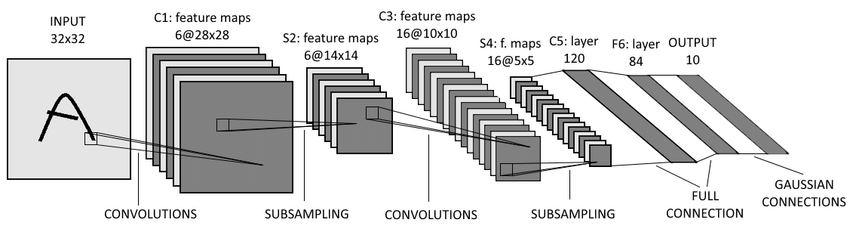
\includegraphics[width=\textwidth]{eiti/lenet5_overview.png}
            \caption{Struktura Modelu LeNet5\cite{LeNet5Diagram}}
       \end{figure}

    \subsection{CIFAR-10}
    Zbiór CIFAR-10 opisany w \textit{Learning Multiple Layers of Features from Tiny Images} \cite{Krizhevsky2009LearningML} zawiera kolorowe obrazy o rozdzielczości 32 na 32 piksele,
    podzielone na 10 klas takich jak np. koń, samolot czy żaba. Podobnie jak zbiór MNIST, CIFAR-10 zawiera
    60,000 obrazów podzielonych na 50,000 przykładów używanych do treningu jak i 10,000 do testowania.
    Aby usunąć problem nadmiernego dopasowania modeli obrazy z zbioru CIFAR10 używane
    do trenowania są losowo modyfikowane. Każdy obraz ma szanse 0.25
    na modyfikacje natężenia, nasycenia, kontrastu oraz odcienia. Dodatkowo każdy obraz może zostać obrócony bądź odbity.

%        \subsubsection{Model Splotowy CIFAR-10}
%        Tutaj w porównaniu do modelu dla zbioru MNIST wykorzystujemy także technikę normalizującą wartości wyjściowe
%        funkcji aktywacji (BatchNorm) w celu zwiększenia stabilności sieci (funkcja aktywacji ReLU nie posiada górnej granicy w
%        przeciwieństwie do funkcji sigmoidalnej). Poniżej znajduje się schemat zastosowanego modelu
        \subsubsection{SimpleNet CIFAR-10}\label{SimpleNetCIFAR-10}
        Model SimpleNet opisany w
        \textit{Lets keep it simple, Using simple architectures to outperform deeper and more complex architectures}\cite{DBLP:journals/corr/HasanPourRVS16}
        jest odpowiedzią na bardziej złożone
        architektury sieci neuronowych (np. InceptionV3~\ref{InceptionV3}), które swoją nieznaczenie wyższą precyzję
        okupywały niewspółmiernie większą złożonością architektury i liczbą parametrów. SimpleNet wykorzystuje klasyczne
        techniki znane z splotowych sieci neuronowych takie jak batch normalization, warstwy splotowe, pooling,
        rektyfikująca funkcja aktywacji czy warstwy Dropout. Skutkiem tego jest model wymagający znacząco mniejszy nakładów
        obliczeniowych. Zarówno przy trenowaniu sieci jak i przy klasyfikacji. Model WRN\cite{DBLP:journals/corr/ZagoruykoK16}
        posiadający 11 milionów parametrów uzyskuje precyzję na poziomie około 95\% dla zbioru CIFAR-10.
        SimpleNet uzyskuje w naszej implementacji precyzję 91.4\% dla około 5 milionów parametrów.
        Autorzy SimpleNet zgłaszał precyzję modelu na poziomie 95.51\% natomiast precyzja na poziomie 91.4\% jest wystarczająca do naszych potrzeb.
        Z uwagi na to że nie jest dostępna oficjalna wersja modelu SimpleNet kompatybilna z tensorflow, konieczne było stworzenie własnej.
        Na Rysunku~\ref{fig:simplenet_cifar10} znajduje się poglądowy schemat architektury modelu SimpleNet.
        \begin{figure}[H]
            \centring
            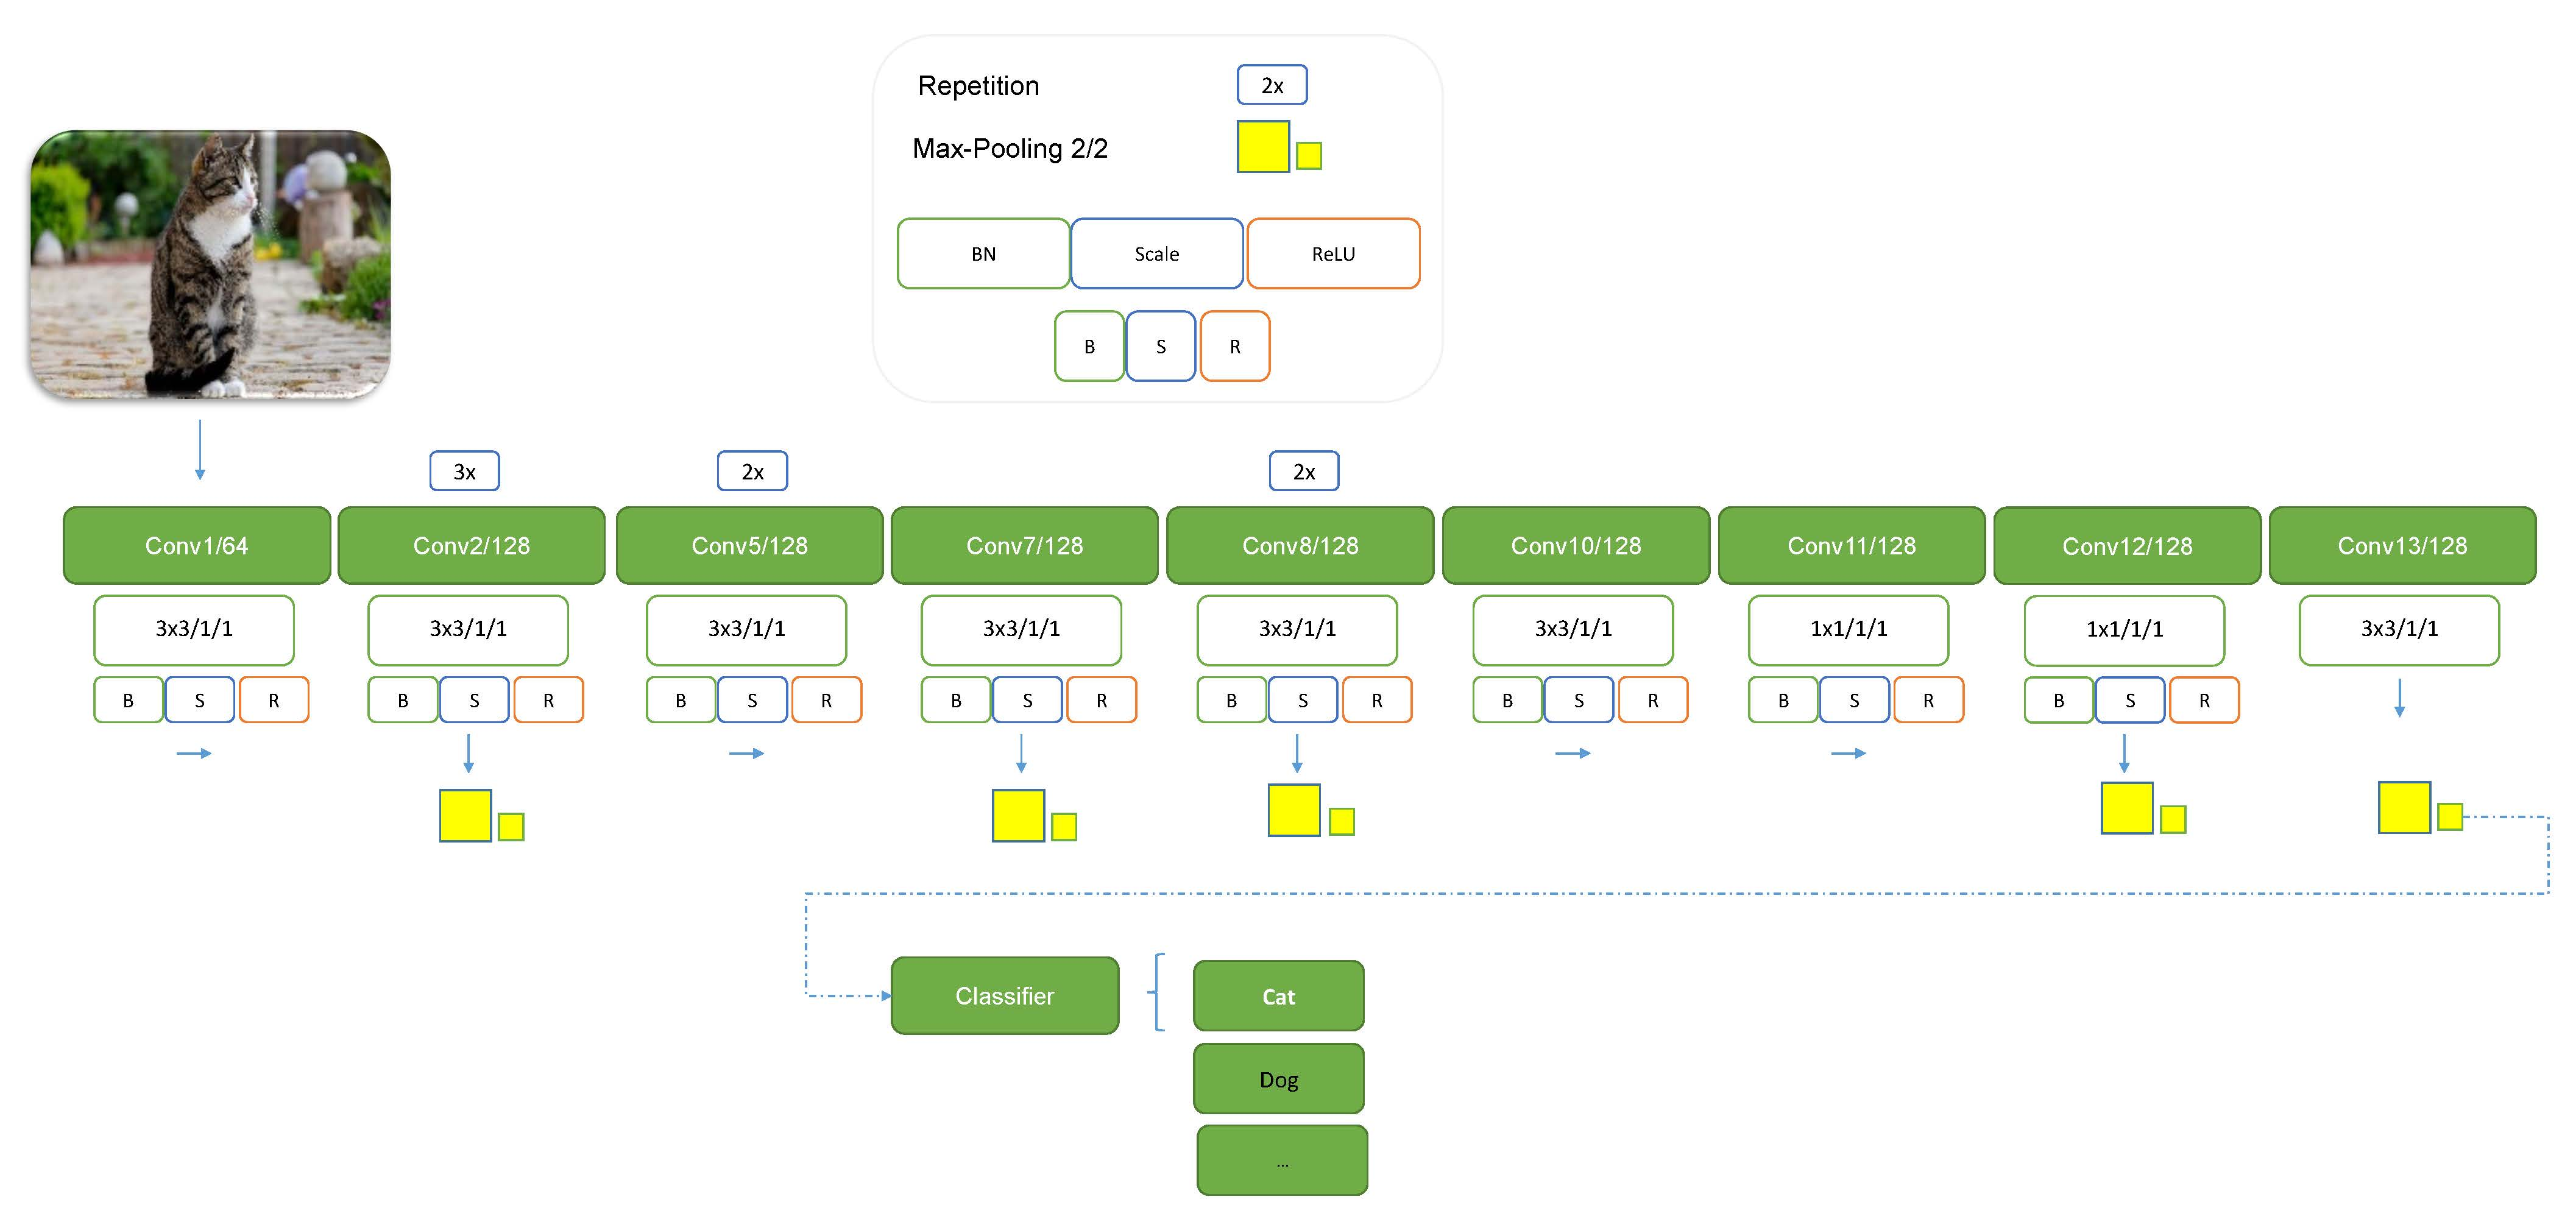
\includegraphics[width=\textwidth]{eiti/simplenet_overview.jpg}
            \caption{Schemat modelu SimpleNet\cite{DBLP:journals/corr/HasanPourRVS16}}
            \label{fig:simplenet_cifar10}
        \end{figure}

    \subsection{CIFAR-100}
    Zbiór CIFAR100 opisany, podobnie jak CIFAR-10 w  \textit{Learning Multiple Layers of Features from Tiny Images} \cite{Krizhevsky2009LearningML}
    jest zbiorem obrazów, o rozdzielczości 32x32 pikseli z trzema kanałami kolorów, podzielonym na 100 klas.
    Każda klasa posiada w tym zbiorze 600 przykładów, z czego 500 jest przykładami treningowymi, a 100 przykładami testowymi.
        \subsubsection{SimpleNet CIFAR-100}\label{SimpleNetCIFAR-100}
        Jako klasyfikator dla zbioru CIFAR-100 wybrany został także model SimpleNet. Architektura sieci i sposób trenowania
        jest identyczny jak w przypadku zbioru CIFAR-10. Jedyną różnicą jest zbiór treningowy którym w tym przypadku jest CIFAR-100.
        Autorzy modelu~\cite{DBLP:journals/corr/HasanPourRVS16} zgłaszają dla zbioru CIFAR-100 precyzję top-1 na poziomie 73.42\%.
        Nasza implementacja uzyskuje precyzję top-1 na poziomie 65.90\% i top-5 na poziomie 89.81\%

%        \subsubsection{Model Splotowy CIFAR-100}
%        Model którego używamy do klasyfikacji obrazów jest analogiczny do modelu użytego w przypadku zbioru CIFAR-10 z jedyną różnicą polegającą na
%        tym że filtry splotowe posiadają większe wymiary. Poniżej znajduje się schemat zastosowanego modelu

    \subsection{ILSVRC2012}\label{ILSVRC2012}
        Zbiór ILSVRC 2012 popularnie nazywany zbiorem ImageNet to, bazowany na bazie danych obrazów ImageNet, zbiór
        przygotowany specjalnie pod konkurs\textit{ImageNet Large Scale Visual Recognition Challenge} \cite{ILSVRC15}.
        Baza danych ImageNet bazuje na bazie WordNet i tworzy hierarchie obrazów uporządkowaną względem synsetów
        czyli zbiorów synonimów (syn od synonim i set z ang. zbiór). Zbiór ILSVRC 2012 posiada 1000 klas i około 1000
        obrazów dla każdej klasy. Obrazy mają rozdzielczośc 299x299 pikseli oraz 3 kanały kolorów. Łącznie zbiór posiada
        1281167 przykładów treningowych oraz 50000 przykładów testowych.

        \subsubsection{InceptionV3}\label{InceptionV3}
            InceptionV3 to zaproponowany przez autorów
            \textit{Rethinking the Inception Architecture for Computer Vision}\cite{DBLP:journals/corr/SzegedyVISW15}
            model którego celem było umożliwienie skalowania architektur modeli splotowych przy ograniczeniu wzrostu
            wymaganej mocy obliczeniowej za pomocą zastosowania warstw "Inception".
            InceptionV3 uzyskuje precyzje top-1 na poziomie 78.8\% oraz precyzję top-5 na
            poziomie 94.4\% dla zbioru ILSVRC~\ref{ILSVRC2012} w implementacji dostarczanej przez bibliotekę Keras.
            Jest to też największy z wykorzystanych modeli. Posiada ponad 23 miliony parametrów oraz 159 warstw.
            \begin{figure}[H]
            \centring
            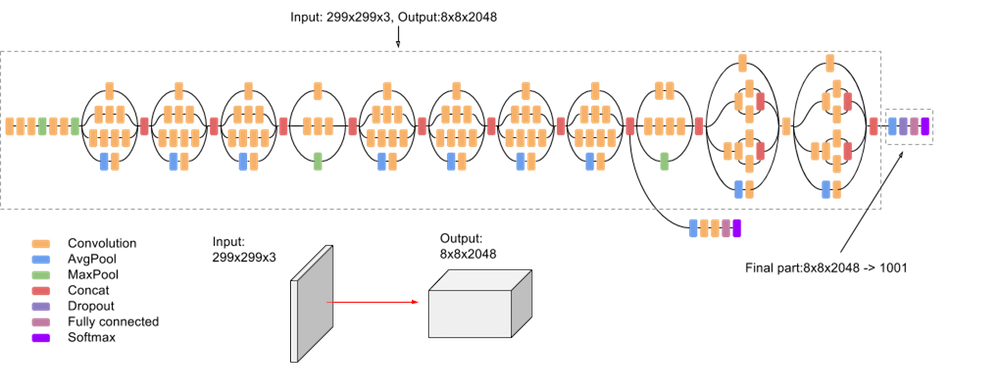
\includegraphics[width=\textwidth]{eiti/inceptionv3overview.png}
            \caption{Schemat modelu InceptionV3}
            \end{figure}

%        \subsubsection{ResNetV2}
%            Autorzy \textit{Identity Mappings in Deep Residual Networks}\cite{DBLP:journals/corr/HeZR016}
%            zaproponowali model należący do grupy modeli nazywanych głębokimi sieciami rezydualnymi (z ang. Deep Residual Networks)
%            nazwany ResNetV2. Jeden z najbardziej złożonych wariantów modelu ResNetV2 - ResNet152
%            uzyskuje precyzję top-1 na poziomie 78.7\% i top-5 94.5\% dla zbioru ILSVRC2012.\ref{ILSVRC2012}.
%            W trakcie pracy, z uwagi na mniejsze wymogi obliczeniowe , użyty został model ResNet50v2, który jest
%            nieco zmniejszoną wersją oryginalnego modelu. Uzyskuje on precyzję top-1 na poziomie 74.9\% i top-5 92.1\%.
%            \begin{figure}[H]
%            \centring
%            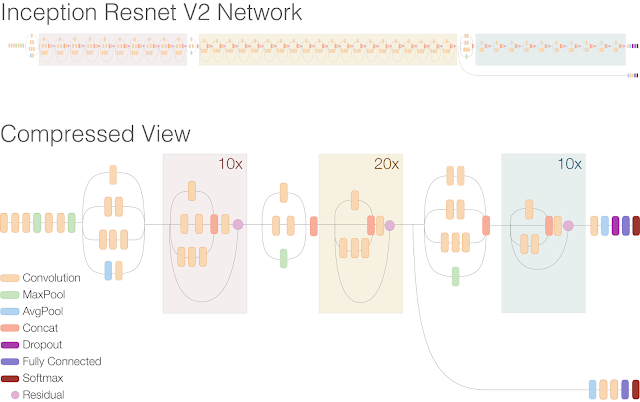
\includegraphics[width=\textwidth]{eiti/resnetv2overview.png}
%            \caption{Schemat modelu ResNetV2}
%            \end{figure}

        \subsubsection{MobileNetV2}\label{MobileNetV2}
            Autorzy \textit{Inverted Residuals and Linear Bottlenecks: Mobile Networks for Classification}\cite{DBLP:journals/corr/abs-1801-04381}
            stworzyli model którego celem, podobnie jak SimpleNet, było zmniejszenie rozmiarów sieci i potrzebnych nakładów obliczeniowych
            do jej używania, przy jednoczesnym zachowaniu wysokiego poziomu precyzji. W tym celu autorzy wykorzystali
            zmodyfikowaną wersję warstw rezydualnych (z ang. residual layer) z takich modeli jak np. ResNet\cite{DBLP:journals/corr/HeZR016}.
            O ile autorzy modelu SimpleNet, starali się uzyskać
            podobny cel dla zbiorów CIFAR-10 i CIFAR-100, tak tutaj autorzy skupili się przede wszystkim na zbiorze ILSVRC.
            MobileNetV2 działa z precyzją top-1 na poziomie 70.6\% i top-5 89.8\% w implementacji dostarczanej przez bibliotekę Keras.
            MobileNetV2 posiada 4.2 miliona parametrów oraz 88 warstw.

            \begin{figure}[H]
            \begin{center}
            \caption{Schemat warstwy \textit{residual bottleneck}\cite{MobileNetV2_GoogleAI_Blogpost}}
            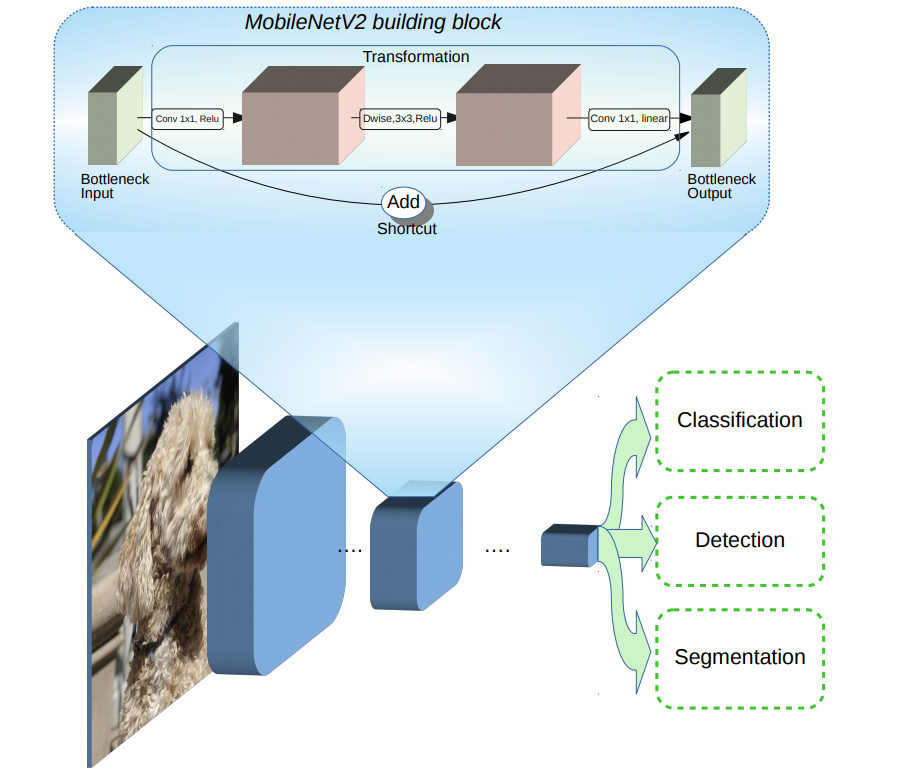
\includegraphics[width=0.6\textwidth]{eiti/mobilenetv2_overview.png}
            \end{center}
            \end{figure}

%            \begin{table}[H]
%            \centering
%            \caption{Tabela z warstwami wykorzystanymi w sieci MobileNetV2}
%            \begin{array}{c|c|c|c|c|c}
%                \text { Input } & \text { Operator } & t & c & n & s \\
%                \hline 224^{2} \times 3 & \text { conv2d } & - & 32 & 1 & 2 \\
%                112^{2} \times 32 & \text { bottleneck } & 1 & 16 & 1 & 1 \\
%                112^{2} \times 16 & \text { bottleneck } & 6 & 24 & 2 & 2 \\
%                56^{2} \times 24 & \text { bottleneck } & 6 & 32 & 3 & 2 \\
%                28^{2} \times 32 & \text { bottleneck } & 6 & 64 & 4 & 2 \\
%                14^{2} \times 64 & \text { bottleneck } & 6 & 96 & 3 & 1 \\
%                14^{2} \times 96 & \text { bottleneck } & 6 & 160 & 3 & 2 \\
%                7^{2} \times 160 & \text { bottleneck } & 6 & 320 & 1 & 1 \\
%                7^{2} \times 320 & \text { conv2d 1x1 } & - & 1280 & 1 & 1 \\
%                7^{2} \times 1280 & \text { avgpool 7x7 } & - & - & 1 & - \\
%                1 \times 1 \times 1280 & \text { conv2d 1x1 } & - & \mathrm{k} & - & \\
%                \hline
%            \end{array}
%            \end{table}

\begin{table}[ht]
\centering
\caption{Precyzja top-1 i top-5 wykorzystywanych przez nas modeli}
\begin{adjustbox}{max width=\textwidth}
\begin{pycode}
from latex_utils import *
generate_accuracy_table_for_all()
\end{pycode}
\end{adjustbox}
\end{table}


\newpage

\section{Wyniki Eksperymentów}\label{comparison}
    W celu oceny skuteczności ataków oraz ich porównania zastosujemy szereg charakterystyk które nam to umożliwią.
    W ramach konferencji
    \textit{Conference on Neural Information Processing Systems} zorganizowany został konkurs którego celem było
    określenie postępu ataków adwersaryjnych oraz wszechstronności modeli zajmujących się przetwarzaniem obrazów\cite{DBLP:journals/corr/abs-1808-01976}.
    W wspomnianym powyżej konkursie zastosowano charakterystykę oceny ataku opisana w następujący sposób:
    \begin{equation}\label{nips_median}
        \text { AQ }=\operatorname{median}\left(\left\{\|q{(\vec{x}, m)} - \vec{x} \|_2 : \vec{x} \in X, m \in M\right\}\right),
    \end{equation}
    gdzie przez \(q(\vec{x}, m)\) rozumiemy złośliwy przykład wygenerowany dla danych wejściowych \(\vec{x}\) i modelu \(m\) przez atak \(q\),
    \(M\) to zbiór wszystkich modeli, a \(X\) to zbiór danych testowych.
    \\~\\
    Ponadto gdy atak nie wygeneruje przykładu adwersaryjnego który jest w stanie oszukać model przypisywana jest górna granica
    metryki \(L_2\).
    Modele które były stosowane w konkursie używały precyzji top-5 która określa procent przykładów których prawdziwa
    kategoria znalazła się wśród pierwszej piątce prawdopodobieństw przypisywanych przez klasyfikator na wyjściu.\\

    Autorzy \textit{Towards Evaluating the Robustness of Neural Networks}\cite{DBLP:journals/corr/CarliniW16a} wykorzystują do oceny swojego ataku precyzję z jaką jest on w stanie oszukać
    model oraz średnią z metryki \(L_2\) różnicy między obrazem oryginalny a złośliwym. Poniżej znajdują się opisy obu metryk:
    \begin{equation}
        \overline{L_2}=\frac{\sum_{\vec{x} \in X}\|q(\vec{x})-\vec{x}\|_2}{|X|}
    \end{equation}

    \begin{equation}
        \text{ACC}=\left\{
        \begin{array}{lc}
        \frac{|\{ \arg \max (f(q(\vec{x}))) \neq y : \vec{x}\in X\}|}{|X|} \text{ gdy \(\vec{\widetilde{y}}\) nie istnieje}\\
        \frac{|\{\arg \max (f(q(\vec{x}))) =\vec{\widetilde{y}} : \vec{x} \in X\}|}{|X|} \text{ w p.p}
        \end{array}
    \end{equation}
    Gdzie \(\arg \max (f(q(\vec{x})))\) to klasa z jaką model klasyfikuje złośliwy przykład \(q(\vec{x})\).
    \\~\\

    Autorzy \textit{DeepFool: a simple and accurate method to fool deep neural networks}\cite{DBLP:journals/corr/Moosavi-Dezfooli15}
    zastosowali średnią wszechstronność (z ang. \textit{robustness}) jako charakterystykę ataku. Można ją sformułować w następujący sposób:

    \begin{equation}
        \rho_{adw}=\frac{1}{|X|}\sum_{\vec{x} \in X} \frac{\|q(\vec{x}) - \vec{x}\|_2}{\|\vec{x}\|_2}
    \end{equation}
    Charakterystyka \(\rho_{adw}\) jest przydatna zwłaszcza w kontekście porównywania ataków dla obrazów należących do
    różnych zbiorów danych gdzie porównanie za pomocą metryki \(L_2\) nie uwzględnia różnicy w ilości atrybutów między zbiorami
    danych.
    Dodatkowo pomocne może być zastosowanie metody opisanej w przykładzie \eqref{nips_median} dla pojedyńczych modeli
    zamiast zestawu wszystkich.

\subsection{Procedura Eksperymentalna}
    We wszystkich eksperymentach odrzucamy przykłady z zbiorów danych które modele klasyfikują niepoprawnie, bądź w
    przypadku ataków z zadaną klasą, takie które które już należą do zadanej klasy. Ataki są wykonywane na przykładach
    wejściowych w transzach (z ang. batches).
Jeśli atak jest atakiem z zadaną klasą $\vec{\widetilde{y}}$, wówczas
    cała transza będzie miała taką samą zadaną klasę $\vec{\widetilde{y}}$ wybraną losowo z prawdopodobieństwem o
    rozkładzie jednostajnym.
Z uwagi na to że wykonanie wszystkich eksperymentów dla całych zbiorów testowych jest w naszym przypadku bardzo czasochłonne,
to liczba przykładów wejściowych na podstawie których obliczamy charakterystyki ataku jest różna i zależna od wymagań obliczeniowych
danego algorytmu. Przy opisie wyników eksperymentów zawieramy także tą informację.
Czas ataku $T$ jest liczony jako średnia z czasu obliczania transzy złośliwych przykładów podzielonego przez liczbe
elementów w transzy.

\subsection{FGSM}\label{FGSM-SCORES}
Jedynym parametrem w klasycznym wariancie metody FGSM jest \(\epsilon\) który określa rozmiar zmiany wprowadzanej dla
    każdego atrybutu. W przypadku obarazów zmiana wartości natężenia każdego kanału dla każdego piksela.
Testy dla wszystkich wariantów ataku FGSM są przeprowadzane dla losowo wybranego 1000 przykładów ze zbioru testowego.
Dla eksperymentów przeprowadzonych na zbiorze ILSVRC2012~\ref{ILSVRC2012} oblicznia są przeprowadzone w transzach po 2 elementy,
    natomiast dla pozostały zbiorów rozmiar transzy to 500 elementów.

%%%%%%%%%%%%%%%%%TABELA%%%%%%%%%%%%%%%%%%%
\begin{table}[ht]
\begin{adjustbox}{max width=\textwidth}
\begin{pycode}
from latex_utils import *
generate_fgsm_table()
\end{pycode}
\end{adjustbox}
\caption{porównanie charakterystyk ataku FGSM względem różnych wartości parametru \(\epsilon\)}
\end{table}
%%%%%%%%%%%%%%%%%TABELA%%%%%%%%%%%%%%%%%%%

\begin{figure}[h]
    \caption{Przykłady złośliwych przykładów wybranych na podstawie obrazów z różnych zbiorów za pomocą metody FGSM}

    \begin{subfigure}[t]{\textwidth}
        \includegraphics[width=\textwidth]{img/row_fgsm_mnist_conv_modelpng.png}
        \caption{MNIST}
        \label{fig:fgsm_mnist_row}
    \end{subfigure}%

    \begin{subfigure}[t]{\textwidth}
        \includegraphics[width=\textwidth]{img/row_fgsm_cifar10_conv_modelpng.png}
        \caption{CIFAR-10}
        \label{fig:fgsm_cifar10_row}
    \end{subfigure}%

    \begin{subfigure}[t]{\textwidth}
        \includegraphics[width=\textwidth]{img/row_fgsm_cifar100_conv_modelpng.png}
        \caption{CIFAR-100}
        \label{fig:fgsm_cifar100_row}
    \end{subfigure}%

    \begin{subfigure}[t]{\textwidth}
        \includegraphics[width=\textwidth]{img/row_fgsm_imagenet_v3png.png}
        \caption{ImageNet}
        \label{fig:fgsm_imagenet_row}
    \end{subfigure}%

\end{figure}



\pagebreak
\subsection{I-FGSM}\label{I-FGSM-SCORES}
Metoda I-FGSM \ref{IFGSM} oprócz parametru \(\epsilon\) kontrolujemy także liczbą iteracji \(i\) w których modyfikujemy
oryginalny obraz.

\begin{table}[ht]
\begin{adjustbox}{max width=\textwidth}
\begin{pycode}
from latex_utils import *
generate_ifgsm_table()
\end{pycode}
\end{adjustbox}
\caption{porównanie charakterystyk ataku I-FGSM dla kilku różnych wartości \(i\) i \(\epsilon\)}
\end{table}

\begin{figure}[H]
    \caption{Przykłady złośliwych przykładów wybranych na podstawie obrazów z różnych zbiorów za pomocą metody I-FGSM}

    \begin{subfigure}[t]{\textwidth}
        \includegraphics[width=\textwidth]{img/row_iterative_fgsm_mnist_conv_modelpng.png}
        \caption{MNIST}
        \label{fig:itertative_fgsm_mnist_row}
    \end{subfigure}%

    \begin{subfigure}[t]{\textwidth}
        \includegraphics[width=\textwidth]{img/row_iterative_fgsm_cifar10_conv_modelpng.png}
        \caption{CIFAR-10}
        \label{fig:itertative_fgsm_cifar10_row}
    \end{subfigure}%

    \begin{subfigure}[t]{\textwidth}
        \includegraphics[width=\textwidth]{img/row_iterative_fgsm_cifar100_conv_modelpng.png}
        \caption{CIFAR-100}
        \label{fig:iterative_fgsm_cifar100_row}
    \end{subfigure}%

    \begin{subfigure}[t]{\textwidth}
        \includegraphics[width=\textwidth]{img/row_iterative_fgsm_imagenet_v3png.png}
        \caption{ImageNet}
        \label{fig:iterative_fgsm_imagenet_row}
    \end{subfigure}%

\end{figure}

\pagebreak
\subsection{LL-FGSM}\label{LL-FGSM-SCORES}
Metoda LL-FGSM oprócz perturbacji \(\epsilon\) oraz liczby iteracji \(i\) pozwala nam na narzucenie klasy z jaką model
ma klasyfikować. Klasy do testów wybierane są losowo z rozkładem jednostajnym.
\begin{table}[h!]
\begin{adjustbox}{max width=\textwidth}
\begin{pycode}
from latex_utils import *
generate_llfgsm_table()
\end{pycode}
\end{adjustbox}
\caption{tabela z charkterystykami dla ataku LL-FGSM dla kilku różnych wartości \(i\) i \(\epsilon\)}
\end{table}

\pagebreak

\begin{figure}[H]
        \includegraphics[width=\textwidth]{img/grid_llfgsm_imagenet_v3.png}
        \caption{Przykładowe złośliwe obrazy z zbioru ILSVRC2012~\ref{ILSVRC2012} uzyskane za pomocą metody LL-FGSM z użyciem parametrów \(\epsilon=0.0005\) i \(i=1000\)}
        \label{fig:imagenet_grid_llfgsm}
\end{figure}

Zestawiając charakterystyki metod I-FGSM(\ref{I-FGSM-SCORES}) i FGSM(\ref{FGSM-SCORES}) można zauważyć że zgodnie z intuicją dotyczącą
algorytmów optymalizacyjnych wykorzystujących gradient większa liczba mniejszych kroków przynosi zwiększoną skuteczność ataku wraz
z mniejszą perturbacją oryginalnego obrazu w sensie różnicy \(\|x-x^{'}\|_2\) obrazu oryginalnego i złośliwego.
Mniejszą skuteczność, rozumianą w sensie precyzji, wariantu LL-FGSM(\ref{LL-FGSM-SCORES}) można tłumaczyć tym że pozostałe warianty
metody FGSM korzystają z gradientu w celu modyfikacji obrazu tak aby zmaksymalizować funkcję kosztu która normalnie zostałaby użyta w procesie nauczania modelu,
natomiast wariant LL-FGSM stara się tak modyfikować obraz aby zminimalizować funkcję kosztu gdzie zamiast faktycznej klasy jest nasza zadana klasa.
Warto też napomnieć że metoda FGSM wykorzystuje metodę propagacji wstecznej w celu obliczenia gradientu obrazu względem elementu wektora wyjściowego w każdej iteracji.
Z tego tytułu ilość obliczeń potrzebnych do uzyskania wyniku rośnie wraz z liczbą iteracji i rozmiarami modelu, co można też zauważyć w przestawionych wcześniej
tabelach.
%\todo{odwołać się do publikacji}


\subsection{L-BFGS-B}
Atak L-BFGS-B wykorzystuje wyszukiwanie binarne w celu znalezienia parametru \(c\) z równania~\ref{l-bfgs-b-equation}.
Dlatego jest nieco bardziej czasochłonna niż metoda FGSM. Możliwe jest przyśpieszenie tej metody poprzez np.
zmniejszenie liczby kroków wyszukiwania binarnego w celu znalezienia parametru \(c\), bądź ustawienia stałej wartości.
Potencjalnie jednak powodowałoby to zmniejszenie precyzji ataku, bądź zwiększenie skali perturbacji rozumianej jako
\(\|x-x'\|_2\)
Identycznie jak dla FGSM rozmiar transzy ILSVRC2012~\ref{ILSVRC2012} to 2, natomiast dla pozostałych zbiorów to 100.
Ekpreymenty są przeprowadzone dla 1000 elementów dla każdego zbioru.

\begin{table}[H]
\caption{Wyniki ataku L-BFGS-B}
\begin{adjustbox}{max width=\textwidth}
\begin{pycode}
from latex_utils import *
generate_bfgs_table()
\end{pycode}
\end{adjustbox}
\end{table}

\begin{figure}[H]
    \includegraphics[width=\textwidth]{img/grid_bfgs_cifar100_conv_model.png}
    \caption{Przykłady wygenerowanych złośliwych przykładów z zadaną klasą za pomocą metody L-BFGS-B dla zbioru CIFAR-100}
    \label{fig:cifar100_grid_bfgs}
\end{figure}


\subsection{GenAttack}
Atak GenAttack posiada 4 parametry które kontrolują jego zachowanie. Jako że atak wykorzstuje techniki
znane z algorytmów genetycznych jesteśmy w stanie kontrolować rozmiar populacji $N$, liczbę generacji $i$, szanse na mutacje
danego osobnika $\alpha$ oraz siłę mutacji $\delta$.
Ta metoda jest stosunkowo czasochłonna, dlatego dokonujemy obliczeń dla 100 elementów z każdego zbioru testowego.
Dla wszystkich zbiorów poza ILSVRC2012~\ref{ILSVRC2012} wykorzystujemy transze o rozmiarze 100 elementów, natomiast dla ILSVRC2012 rozmiar transzy to 2.
Dodatkowo autorzy oryginalnej publikacji proponują używanie znacząco większej liczby generacji niż 1000 które zostało użyte w naszych eksperymentach.

\begin{table}[h]
\begin{adjustbox}{max width=\textwidth}
\begin{pycode}
from latex_utils import *
generate_getattack_table()
\end{pycode}
\end{adjustbox}
\caption{porównanie charakterystyk ataku GenAttack dla różnych modeli}
\end{table}

\begin{figure}[H]
    \caption{Przykłady wygenerowanych złośliwych przykładów z zadaną klasą za pomocą metody GenAttack}

    \begin{subfigure}[t]{0.48\textwidth}
        \includegraphics[width=\textwidth]{img/side_by_side_genattackmnist_tf_model.png}
        \caption{MNIST TF}
        \label{fig:mnist_side_genattack}
    \end{subfigure}%
    \hfill
    \begin{subfigure}[t]{0.48\textwidth}
        \includegraphics[width=\textwidth]{img/side_by_side_genattacksimplenet_cifar10.png}
        \caption{SimpleNet CIFAR-10}
        \label{fig:cifar10_side_genattack}
    \end{subfigure}%

    \begin{subfigure}[t]{0.48\textwidth}
        \includegraphics[width=\textwidth]{img/side_by_side_genattacksimplenet_cifar100.png}
        \caption{SimpleNet CIFAR-100}
        \label{fig:cifar100_side_genattack}
    \end{subfigure}%
    \hfill
    \begin{subfigure}[t]{0.48\textwidth}
        \includegraphics[width=\textwidth]{img/side_by_side_genattackimagenet_v3.png}
        \caption{InceptionV3}
        \label{fig:imagenet_side_genattack}
    \end{subfigure}%

\end{figure}



Podobnie jak w większości algorytmów ewolucyjnych skuteczność metody GenAttack zależy od rozmiaru populacji oraz liczby
i liczby generacji jaką przejdzie. Liczba atrybutów danych wejściowych wpływa na liczbę dokonywanych operacji. Dlatego też złośliwe przykłady dla zbiorów pokroju
ILSVRC2012~\ref{ILSVRC2012} wymagają więcej czasu do wygenerowania niż przykłady ze zbioru MNIST.

\subsection{DeepFool}
Deepfool jest atakiem bez zadanej klasy. Jedynym tak naprawdę kontrolowanym przez nas parametrem jest maksymalna
liczba iteracji jaką wykona atak jeśli nie uda mu się utworzyć złośliwego przykładu obrazu. Identycznie jak dla FGSM rozmiar transzy ILSVRC2012~\ref{ILSVRC2012} to 2, natomiast dla pozostałych zbiorów to 100.
Eksperymenty są przeprowadzone dla 1000 elementów dla każdego zbioru.


\begin{table}[h]
\begin{adjustbox}{max width=\textwidth}
\begin{pycode}
from latex_utils import *
generate_deepfool_table()
\end{pycode}
\end{adjustbox}
\caption{porównanie charakterystyk ataku DeepFool dla różnych modeli}
\end{table}

\begin{figure}[H]
    \caption{Przykłady wygenerowanych złośliwych za pomocą metody DeepFool}

    \begin{subfigure}[t]{0.48\textwidth}
        \includegraphics[width=\textwidth]{img/side_by_side_deepfoolmnist_tf_model.png}
        \caption{MNIST TF}
        \label{fig:mnist_side_deepfool}
    \end{subfigure}%
    \hfill
    \begin{subfigure}[t]{0.48\textwidth}
        \includegraphics[width=\textwidth]{img/side_by_side_deepfoolsimplenet_cifar10.png}
        \caption{SimpleNet CIFAR-10}
        \label{fig:cifar10_side_deepfool}
    \end{subfigure}%

    \begin{subfigure}[t]{0.48\textwidth}
        \includegraphics[width=\textwidth]{img/side_by_side_deepfoolsimplenet_cifar100.png}
        \caption{SimpleNet CIFAR-100}
        \label{fig:cifar100_side_deepfool}
    \end{subfigure}%
    \hfill
    \begin{subfigure}[t]{0.48\textwidth}
        \includegraphics[width=\textwidth]{img/side_by_side_deepfoolimagenet_v3.png}
        \caption{InceptionV3}
        \label{fig:imagenet_side_deepfool}
    \end{subfigure}%

\end{figure}

\subsection{Carlini \& Wagner}
Metoda którą zaproponowali Carlini i Wagner w \textit{Towards Evaluating the Robustness of Neural Networks}\cite{DBLP:journals/corr/CarliniW16a}
wykorzystuje znane metody optymalizacji stosowane w dziedzinie nauczania maszynowego. W celu uzyskania poniższych wyników zasotosowana została
Adam\cite{DBLP:journals/corr/KingmaB14}. Identycznie jak dla FGSM rozmiar transzy ILSVRC2012~\ref{ILSVRC2012} to 2, natomiast dla pozostałych zbiorów to 100.
Ekpreymenty są przeprowadzone dla 1000 elementów dla każdego zbioru. W poniższej tabli $i$ oznacza liczbę iteracji optymalizacji równania (~\ref{eq:c_and_w}),
natomiast $i_b$ to liczba kroków wykonana wyszukiwania binarnego w celu znalezienia parametru $c$ z równania (~\ref{eq:c_and_w}).

\begin{table}[h]
\begin{adjustbox}{max width=\textwidth}
\begin{pycode}
from latex_utils import *
generate_carlini_table()
\end{pycode}
\end{adjustbox}
\caption{porównanie charakterystyk ataku Carlini & Wagner dla różnych wartości parametrów}
\end{table}


\begin{figure}[H]
    \caption{Przykłady wygenerowanych złośliwych przykładów z zadaną klasą za pomocą metody Carlini Wagner dla parametrów
        optimization\_iter=1000, binary\_iter=10, c\_high=100.0, c\_low=0.0, \(\kappa=0.0\)}

    \begin{subfigure}[t]{0.48\textwidth}
        \includegraphics[width=\textwidth]{img/side_by_side_carlinimnist_tf_model.png}
        \caption{MNIST TF}
        \label{fig:mnist_side_carlini}
    \end{subfigure}%
    \hfill
    \begin{subfigure}[t]{0.48\textwidth}
        \includegraphics[width=\textwidth]{img/side_by_side_carlinisimplenet_cifar10.png}
        \caption{SimpleNet CIFAR-10}
        \label{fig:cifar10_side_carlini}
    \end{subfigure}%

    \begin{subfigure}[t]{0.48\textwidth}
        \includegraphics[width=\textwidth]{img/side_by_side_carlinisimplenet_cifar100.png}
        \caption{SimpleNet CIFAR-100}
        \label{fig:cifar100_side_carlini}
    \end{subfigure}%
    \hfill
    \begin{subfigure}[t]{0.48\textwidth}
        \includegraphics[width=\textwidth]{img/side_by_side_carliniimagenet_v3.png}
        \caption{InceptionV3}
        \label{fig:imagenet_side_carlini}
    \end{subfigure}%

\end{figure}


\subsection{JSMA}
Jako że metoda JSMA w dowolnym wariancie, poza M-JSMA, wymaga rozpatrzenia wszystkich możliwych par atrybutów jej wykorzystanie dla
zbioru ILSVRC2012~\ref{ILSVRC2012} jest niepraktyczne jako że wymagałoby od nas w każdym kroku ewaluacji
$\binom{299*299*3}{2} = 4479002052528$ możliwych par. W przypadku wariantu M-JSMA byłoby to $8958004105056‬$ par jako że rozpatrujemy zarówno $S^-() \text{ jak i } S^+()$.
Dlatego też w poniższych rozważaniach wykluczone są wszystkie modele wytrenowane na powyższym zbiorze.
Dla wszystkich pozostałych zbiorów wykorzystujemy transze po 10 elementów i testujemy w sumie 1000 elementów.
\begin{table}[h]
\begin{adjustbox}{max width=\textwidth}
\begin{pycode}
from latex_utils import *
generate_jsma_table()
\end{pycode}
\end{adjustbox}
\caption{Charakterystyki ataku JSMA+ dla różnych modeli}
\end{table}

\begin{figure}[H]
    \caption{Przykłady wygenerowanych złośliwych przykładów z zadaną klasą za pomocą metody JSMA-F+ dla parametrów
        \(\delta_{max} = 0.1\) i \(\theta = 1.0\)}
    \begin{subfigure}[t]{0.48\textwidth}
        \includegraphics[width=\textwidth]{img/side_by_side_jsma_targetedmnist_tf_model.png}
        \caption{MNIST TF}
        \label{fig:mnist_side_jsma_targeted}
    \end{subfigure}%
    \hfill
    \begin{subfigure}[t]{0.48\textwidth}
        \includegraphics[width=\textwidth]{img/side_by_side_jsma_targetedsimplenet_cifar10.png}
        \caption{SimpleNet CIFAR-10}
        \label{fig:cifar10_side_jsma_targeted}
    \end{subfigure}%

    \begin{subfigure}[t]{0.48\textwidth}
        \includegraphics[width=\textwidth]{img/side_by_side_jsma_targetedsimplenet_cifar100.png}
        \caption{SimpleNet CIFAR-100}
        \label{fig:cifar100_side_jsma_targeted}
    \end{subfigure}%
    \hfill
\end{figure}



\newpage




%%%%%%%%%%%%%%%% BIBLIOGRAFIA %%%%%%%%%%%%%%%%%

\cleardoublepage
\bibliography{pdi}
\bibliographystyle{ieeetr}

%%%%%%%%%%%%%%%% BIBLIOGRAFIA %%%%%%%%%%%%%%%%%

%%%%%%%%%%%%%%%% SPIS %%%%%%%%%%%%%%%%%%%%%%%%%
\newpage
\pagestyle{plain}

% Wykaz symboli i skrótów.
% Pamiętaj, żeby posortować symbole alfabetycznie
% we własnym zakresie. Ponieważ mało kto używa takiego wykazu,
% uznałem, że robienie automatycznie sortowanej listy
% na poziomie LaTeXa to za duży overkill.
% Makro \acronymlist generuje właściwy tytuł sekcji,
% w zależności od języka.
% Makro \acronym dodaje skrót/symbol do listy,
% zapewniając podstawowe formatowanie.
% //AB
\vspace{0.8cm}

\acronymlist

\acronym{$\vec{x}$}{wektor}
\acronym{$\vec{x'}$}{spreparowany przez atak złośliwy przykład }
\acronym{$\vec{r}$}{perturbacja wprowadzona do oryginalnego przykładu w celu uzyskania złośliwego przykładu $\vec{x'}=\vec{x}+\vec{r}$}
\acronym{$\vec{x}_i$}{i-ty element wektora $\vec{x}$}
\acronym{$\vec{x}^i$}{i-ty wektor}
%\acronym{$f(\vec{x})$}{funkcja opisująca model klasyfikacyjny}
\acronym{$f_i(\vec{x})$}{i-ty element wektora, będącego wektorem wyjściowym modelu, opisującego prawdopodobieństwo należenia do danej klasy $i$}
\acronym{$q(\vec{x}, f)$}{atak $q$ zastosowany na przykładzie $\vec{x}$ i modelu opisanego funkcją $f$}
\acronym{$X$}{zbiór danych dla którego $\vec{x} \in X$}
\acronym{$y$}{prawdziwa klasa do której należy przykład $\vec{x}$}
\acronym{$\widetilde{y}$}{narzucona przez atakującego klasa do której ma należeć spreparowany przykład $x'$}
\acronym{$\widehat{y}$}{klasa przypisana przykładowi wejściowemu przez model klasyfikacyjny taka że $\widehat{y} = \argmax f(\vec{x})$}
%\acronym{$N$}{Rozmiar populacji w algorytmie genetycznym}

\listoffigurestoc     % Spis rysunków.
\vspace{1cm}          % vertical space
\listoftablestoc      % Spis tabel.
\vspace{1cm}          % vertical space
\listofappendicestoc  % Spis załączników

%%%%%%%%%%%%%%%% SPIS %%%%%%%%%%%%%%%%%%%%%%%%%
\appendix{Pozostałe przykłady ataków}

%%%%%%%%%%%%%%%%%%LL-FGSM%%%%%%%%%%%%%%%%%%%%%%%%%%%%%%%%%%%%%
\begin{figure}[H]
    \centering
    \includegraphics[width=\textwidth]{img/grid_llfgsm_mnist_conv_model.png}
    \caption{Przykładowe złośliwe obrazy z zbioru CIFAR-10 uzyskane za pomocą metody LL-FGSM}
    \label{fig:mnist_grid_llfgsm}
\end{figure}%

\begin{figure}[H]
    \centering
    \includegraphics[width=\textwidth]{img/grid_llfgsm_cifar10_conv_model.png}
    \caption{Przykładowe złośliwe obrazy z zbioru CIFAR-100 uzyskane za pomocą metody LL-FGSM}
    \label{fig:cifar10_grid_llfgsm}
\end{figure}
%%%%%%%%%%%%%%%%%%%%%%%%%%%%%%%%%%%%%%%%%%%%%%%%%%%%%%%%%%%%%%%%%

%%%%%%%%%%%%%%%%%%L-BFGS-B%%%%%%%%%%%%%%%%%%%%%%%%%%%%%%%%%%
\begin{figure}[H]
    \centering
    \includegraphics[width=\textwidth]{img/grid_bfgs_mnist_conv_model.png}
    \caption{Przykładowe złośliwe obrazy z zbioru MNIST uzyskane za pomocą metody L-BFGS-B}
\end{figure}
\begin{figure}[H]
    \centering
    \includegraphics[width=\textwidth]{img/grid_bfgs_cifar10_conv_model.png}
    \caption{Przykładowe złośliwe obrazy z zbioru CIFAR-10 uzyskane za pomocą metody L-BFGS-B}
\end{figure}
%%%%%%%%%%%%%%%%%%%%%%%%%%%%%%%%%%%%%%%%%%%%%%%%%%%%%%%%%%%%%

\end{document}
